\noindent Die Wahrscheinlichkeitstheorie ist ein mathematisches Modell zur Beschreibung empirischer Sachverhalte, bei denen der Zufall eine Rolle spielt. Sie entstand aus dem Wunsch, die Gewinnaussichten bei Gl\"{u}cksspielen zu prognostizieren. Aber schon bald zeigte sich, dass sie in sehr vielen anderen Gebieten angewendet werden kann, zum Beispiel im Versicherungswesen oder in der Mess- und Prozesstechnik. Der Versuch, den Begriff der Wahrscheinlichkeit zu definieren, f\"{u}hrt zun\"{a}chst zum klassischen Wahrscheinlichkeitsbegriff von Laplace. Diese Definition ist allerdings f\"{u}r Anwendungen in der Mess- und Prozesstechnik zu speziell und wird deshalb verallgemeinert.
\subsection{Grundbegriffe und Mengenoperationen}
\noindent Bevor die Grundlagen der Wahrscheinlichkeitstheorie zusammengestellt und diskutiert werden k\"{o}nnen, m\"{u}ssen einige Grundbegriffe erl\"{a}utert und die Grundz\"{u}ge der Mengenlehre eingef\"{u}hrt werden. Zur Veranschaulichung der Begriffe wird parallel ein W\"{u}rfelexperiment beschrieben.
\subsubsection{Ereignisse}
\noindent Die Wahrscheinlichkeitstheorie hat den Anspruch, die Wahrscheinlichkeit f\"{u}r den Ausgang von zuf\"{a}lligen Prozessen vorauszusagen. Der Zufallsprozess wird auch als Zufallsexperiment bezeichnet. Er muss wiederholbar und das Ergebnis vom Zufall abh\"{a}ngig sein. Das konkrete Ergebnis kann im Voraus nicht eindeutig bestimmt werden.\newline
\noindent Bekanntestes Beispiel f\"{u}r ein Zufallsexperiment ist das Werfen eines regelm\"{a}{\ss}igen W\"{u}rfels. Der W\"{u}rfel kann beliebig oft geworfen werden und das Ergebnis ist nicht vorhersagbar. Bei jedem Zufallsexperiment sind unterschiedliche Ergebnisse m\"{o}glich, die zuf\"{a}llig eintreffen. Diese Ergebnisse werden Zufallsereignisse oder Ereignisse genannt. Beim einmaligen Werfen eines W\"{u}rfels k\"{o}nnen die Ereignisse

\begin{equation}\label{eq:twoone}
1, 2, 3, 4, 5 \text{ oder } 6
\end{equation}

\noindent eintreffen oder realisiert werden. Im Folgenden werden unterschiedliche Ereignisse definiert, die sich aus einem Zufallsexperiment ergeben k\"{o}nnen. Als Beispiel dient dabei das einmalige W\"{u}rfeln mit einem W\"{u}rfel.\bigskip

{\fontfamily{phv}\selectfont
\noindent\textbf{Elementarereignis}} \smallskip

\noindent Sind Ergebnisse von Zufallsexperimenten nicht weiter zerlegbar und schlie{\ss}en sich gegenseitig aus, werden sie als Elementarereignisse bezeichnet. Beim einmaligen W\"{u}rfeln sind die Ereignisse 

\begin{equation}\label{eq:twotwo}
1, 2, 3, 4, 5 \text{ oder } 6
\end{equation}

\noindent Elementarereignisse. Sie bestehen aus einem Element und sind deshalb nicht weiter zerlegbar, au{\ss}erdem schlie{\ss}en sie sich gegenseitig aus.

\clearpage

{\fontfamily{phv}\selectfont
\noindent\textbf{Ereignisraum}} \smallskip

\noindent  Die Menge $\Omega$ aller Elementarereignisse eines Zufallsexperimentes wird als Ereignisraum dieses Zufallsexperimentes bezeichnet. In der Literatur wird der Ereignisraum auch Grundraum genannt. F\"{u}r das einmalige W\"{u}rfeln ergibt sich ein Ereignisraum $\Omega$ von

\begin{equation}\label{eq:twothree}
\Omega = \left\{1, 2, 3, 4, 5, 6\right\}
\end{equation}

\noindent Dabei werden, wie in der Mengenlehre \"{u}blich, Mengen mit geschweiften Klammern dargestellt. \bigskip

{\fontfamily{phv}\selectfont
\noindent\textbf{Ereignismenge}} \smallskip

\noindent Eine Menge m\"{o}glicher Elementarereignisse wird als Ereignismenge A bezeichnet. Sie ist eine Teilmenge des Ereignisraums $\Omega$. Zum Beispiel ist beim einmaligen W\"{u}rfeln die Menge A der geraden Zahlen 

\begin{equation}\label{eq:twofour}
A = \left\{2, 4, 6\right\}
\end{equation}

\noindent eine Teilmenge des Ereignisraums $\Omega$ und damit eine Ereignismenge.\bigskip

{\fontfamily{phv}\selectfont
\noindent\textbf{Unm\"{o}gliches Ereignis}} \smallskip

\noindent Ist ein Ereignis kein Teilelement des Ereignisraums, wird es als unm\"{o}gliches Ereignis U bezeichnet. 

\begin{equation}\label{eq:twofive}
A\not\subset \Omega 
\end{equation}

\noindent Beim einmaligen W\"{u}rfeln kann die Zahl 7 nicht eintreffen, das Ereignis ist unm\"{o}glich. \bigskip

{\fontfamily{phv}\selectfont
\noindent\textbf{Sicheres Ereignis}} \smallskip

\noindent Entspricht die Definition eines Ereignisses dem gesamten Ereignisraum $\Omega$,

\begin{equation}\label{eq:twosix}
A=\Omega 
\end{equation}

\noindent wird das Ereignis als sicheres Ereignis S bezeichnet. Bei dem W\"{u}rfeln mit einem W\"{u}rfel wird eines der Ergebnisse 1, 2, 3, 4, 5 oder 6 sicher eintreffen.

\subsubsection{Verkn\"{u}pfungen von Ereignissen durch Mengenoperationen}

\noindent Eine Menge kann, wie im vorhergehenden Abschnitt gezeigt wird, als eine Zusammenfassung verschiedener Ereignisse verstanden werden. Zufallsereignisse lassen sich daher mithilfe der Mengenlehre beschreiben und verkn\"{u}pfen. Der Mengenbegriff wird anhand des Zufallsexperimentes W\"{u}rfeln mit einem regelm\"{a}{\ss}igen W\"{u}rfel verdeutlicht. Das W\"{u}rfeln f\"{u}hrt zu sechs m\"{o}glichen Ereignissen. Diese M\"{o}glichkeiten bilden den Ereignisraum ?, der als Menge dargestellt werden kann.

\begin{equation}\label{eq:twoseven}
\Omega = \left\{1, 2, 3, 4, 5, 6\right\}
\end{equation}

\noindent F\"{u}r das Experiment werden die Mengen A - D definiert:

\begin{itemize}
    \item[] A \qquad Würfeln einer geraden Zahl, $A = \left \{ 2,4,6 \right \}$  
    \item[] B \qquad Würfeln einer durch 3 teilbaren Zahl, $B = \left \{ 3,6 \right \}$
    \item[] C \qquad Würfeln einer 1, $C = \left \{ 1 \right \}$  
    \item[] D \qquad Würfeln einer 4, $D = \left \{ 4 \right \}$ 
\end{itemize}

\noindent Die Ereignisse sind in Bild \ref{fig:Mengen} grafisch dargestellt:

\noindent 
\begin{figure}[H]
  \centerline{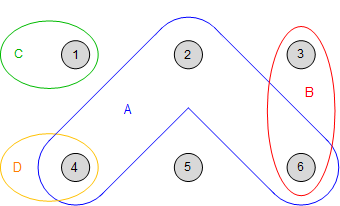
\includegraphics[width=0.5\textwidth]{Kapitel2/Bilder/image1}}
  \caption{Darstellung des Zufallsexperimentes Wurf eines regelm\"{a}{\ss}igen W\"{u}rfels}
  \label{fig:Mengen}
\end{figure}

\noindent Mit dem Beispiel Wurf eines regelm\"{a}{\ss}igen W\"{u}rfels werden im Folgenden die grundlegenden Mengenoperationen beschrieben. \bigskip

{\fontfamily{phv}\selectfont
\noindent\textbf{Element der Menge}} \smallskip

\noindent Ist eine Menge D in einer Menge A vollst\"{a}ndig enthalten, wird sie als Element der Menge bezeichnet. Die Eigenschaft wird mit der Schreibweise 

\begin{equation}\label{eq:twoeight}
D\in A
\end{equation}

\noindent dargestellt. Ist die Menge C kein Element der Menge A, ergibt sich die Schreibweise

\begin{equation}\label{eq:twonine}
C\notin A
\end{equation}

{\fontfamily{phv}\selectfont
\noindent\textbf{Teilmenge}} \smallskip

\noindent Ist eine Menge D komplett in einer anderen Menge A enthalten, ist die Menge D eine Teilmenge von der Menge A. Dafür wird die Schreibweise 

\begin{equation}\label{eq:twoten}
D\in A
\end{equation}

\noindent verwendet. \bigskip

{\fontfamily{phv}\selectfont
\noindent\textbf{Vereinigungsmenge}} \smallskip

\noindent Mit $A \cup B$ wird das Ereignis bezeichnet, bei dem das Ereignis A oder das Ereignis B eintrifft. In der Mengenlehre wird von der Vereinigungsmenge der Ereignisse A und B gesprochen. In dem Beispiel aus Bild \ref{fig:Mengen}  umfasst die Vereinigungsmenge $A \cup B$ die Elemente 

\begin{equation}\label{eq:twoeleven}
A\cup B=\left\{2, 3, 4, 6\right\}
\end{equation}

\noindent Die Vereinigungsmenge $A \cup B$ der Ereignisse A und B sind also W\"{u}rfe mit den Augenzahlen 2, 3, 4 oder 6. \bigskip

{\fontfamily{phv}\selectfont
\noindent\textbf{Schnittmenge}} \smallskip

\noindent Mit A $\cap$ B wird das Ereignis bezeichnet, bei dem das Ereignis A und das Ereignis B zusammen eintreffen. In der Mengenlehre wird von der Schnittmenge der Ereignisse A und B gesprochen. In dem Beispiel aus Bild \ref{fig:Mengen} umfasst die Schnittmenge A $\cap$ B das Element 

\begin{equation}\label{eq:twotwelve}
A\cap B=\left\{6\right\}
\end{equation}

\noindent Die Schnittmenge A $\cap$ B der Ereignisse A und B ist ein Wurf mit einer Augenzahl 6. Diese Augenzahl erf\"{u}llt sowohl die Forderung nach einer geraden Zahl als auch die Forderung, durch 3 teilbar zu sein. \bigskip

{\fontfamily{phv}\selectfont
\noindent\textbf{Differenzmenge}} \smallskip

\noindent Die Differenzmenge A{\textbackslash}B ist die Menge aller Elemente, die in A, aber nicht in B vorkommen. F\"{u}r das Beispiel aus Bild \ref{fig:Mengen} ergibt sich die Differenzmenge A{\textbackslash}B zu

\begin{equation}\label{eq:twothirteen}
A\backslash B=\left\{2, 4\right\}
\end{equation}

{\fontfamily{phv}\selectfont
\noindent\textbf{Komplement\"{a}re oder inverse Menge}} \smallskip

\noindent Die komplement\"{a}re oder inverse Menge A' bezeichnet die Ereignisse, die im Ereignisraum liegen, aber kein Element der Menge A sind. 

\begin{equation}\label{eq:twofourteen}
A'=\Omega \backslash A
\end{equation}

\noindent In dem Beispiel aus Bild \ref{fig:Mengen} ergibt sich die komplement\"{a}re Menge A' zu

\begin{equation}\label{eq:twofifteen}
A'=\Omega \backslash A=\left\{1, 3, 5\right\}
\end{equation}

{\fontfamily{phv}\selectfont
\noindent\textbf{Disjunkte Menge}} \smallskip

\noindent Wenn zwei Ereignisse nicht gemeinsam eintreffen k\"{o}nnen, schlie{\ss}en sich die Ereignisse gegenseitig aus. Ihre Schnittmenge ist eine leere Menge.

\begin{equation}\label{eq:twosixteen}
A\cap C=\left\{ \; \right\}
\end{equation}

\noindent Die Mengen werden als disjunkte Mengen bezeichnet. In dem Beispiel aus Bild \ref{fig:Mengen} schlie{\ss}en sich die Ereignisse A und C gegenseitig aus, weil die Zahl 1 keine gerade Zahl ist.\bigskip

{\fontfamily{phv}\selectfont
\noindent\textbf{Rechenregeln f\"{u}r Mengen}} \smallskip

\noindent Mithilfe von Mengenoperationen lassen sich Rechenregeln f\"{u}r die mit den Ereignissen verbundenen Wahrscheinlichkeiten ableiten. Die Rechenregeln sind in Tabelle \ref{tab:twoone} zusammengestellt. Ihre G\"{u}ltigkeit kann anhand des Beispiels des einmaligen W\"{u}rfelns plausibilisiert werden.

\begin{table}[H]
\setlength{\arrayrulewidth}{.1em}
\caption{Funktionen zur Beschreibung von Einschwingvorgängen}
\setlength{\fboxsep}{0pt}%
\colorbox{lightgray}{%
\arrayrulecolor{white}%
\begin{tabular}{| c | c |}
\hline
\parbox[c][0.28in][c]{3.3in}{\smallskip\centering\textbf{\fontfamily{phv}\selectfont{Gesetz}}} & 
\parbox[c][0.28in][c]{3.3in}{\smallskip\centering\textbf{\fontfamily{phv}\selectfont{Rechenoperation}}}\\ \hline

\parbox[c][0.4in][c]{3.3in}{\centering{\fontfamily{phv}\selectfont{Kommutativgesetz}}} &
\parbox[c][0.4in][c]{3.3in}{\centering{$A\cap B=B\cap A, A\cup B=B\cup A$}}\\ \hline

\parbox[c][0.64in][c]{3.3in}{\centering{\fontfamily{phv}\selectfont{Assoziativgesetz}}} & 
\parbox[c][0.64in][c]{3.3in}{\centering{$\left(A\cap B\right)\cap C=A\cap \left(B\cap C\right)$\\
$\left(A\cup B\right)\cup C=A\cup \left(B\cup C\right)$}}\\ \hline

\parbox[c][0.64in][c]{3.3in}{\centering{\fontfamily{phv}\selectfont{Distributivgesetz}}} & 
\parbox[c][0.64in][c]{3.3in}{\centering{$\left(A\cup B\right)\cap C=\left(A\cap C\right)\cup \left(B\cap C\right)$\\
$\left(A\cap B\right)\cup C=\left(A\cup C\right)\cap \left(B\cup C\right)$}}\\ \hline

\parbox[c][0.4in][c]{3.3in}{\centering{\fontfamily{phv}\selectfont{Die Morgansche Regeln}}} &
\parbox[c][0.4in][c]{3.3in}{\centering{$\left(A\cup B\right)'=A'\cap B', \left(A\cap B\right)'=A'\cup B'$}}\\ \hline

\end{tabular}%
}
\label{tab:twoone}
\end{table}

\clearpage

\subsection{Klassische Wahrscheinlichkeit nach Laplace}
\subsubsection{Definition}

\noindent Zur Herleitung des Begriffes der klassischen Wahrscheinlichkeit nach Laplace wird wieder das Beispiel des W\"{u}rfelns mit einem regelm\"{a}{\ss}igen W\"{u}rfel betrachtet. Alle sechs Elementarereignisse schlie{\ss}en einander aus. Da der W\"{u}rfel regelm\"{a}{\ss}ig ist, ist keines dieser sechs Elementarereignisse wahrscheinlicher als ein anderes. Alle Elementarereignisse sind m\"{o}glich und gleich wahrscheinlich. \newline

\noindent In \"{a}hnlicher Weise k\"{o}nnen auch f\"{u}r andere Zufallsexperimente die jeweiligen Elementarereignisse angegeben werden, die einander ausschlie{\ss}en und gleich wahrscheinlich sind. Diese beiden Eigenschaften sind die Voraussetzung f\"{u}r die klassische Wahrscheinlichkeitsrechnung nach Laplace.\newline

\noindent Gibt es bei einem Experiment N gleichwahrscheinliche F\"{a}lle, k\"{o}nnen diese F\"{a}lle in zwei Gruppen eingeteilt werden. Die g\"{u}nstigen F\"{a}lle erf\"{u}llen eine definierte Bedingung, die ung\"{u}nstigen F\"{a}lle erf\"{u}llen die definierte Bedingung nicht. Zum Beispiel kann die Bedingung f\"{u}r ein g\"{u}nstiges Ereignis A lauten, dass bei einem Wurf mit einem regelm\"{a}{\ss}igen W\"{u}rfel eine gerade Zahl gew\"{u}rfelt wird. Dann ist der Wurf mit der Augenzahl 2, 4 oder 6 ein g\"{u}nstiger Fall, alle anderen Augenzahlen sind ung\"{u}nstige F\"{a}lle. \newline

\noindent Wird die Anzahl der g\"{u}nstigen Elementarereignisse mit G bezeichnet und die Anzahl der m\"{o}glichen F\"{a}lle mit N, ergibt sich die Wahrscheinlichkeit P(A) f\"{u}r das g\"{u}nstige Ereignis A nach Laplace zu

\begin{equation}\label{eq:twoseventeen}
P(A)=\dfrac{G}{N} 
\end{equation}

\noindent Das Ereignis A, bei einem Wurf mit einem regelm\"{a}{\ss}igen W\"{u}rfel eine gerade Zahl zu w\"{u}rfeln, ergibt sich aus 3 g\"{u}nstigen Elementarereignissen, n\"{a}mlich den Augenzahlen 2, 4 und 6. Entsprechend ergibt sich f\"{u}r die Wahrscheinlichkeit P(A)

\begin{equation}\label{eq:twoeightteen}
P(A)=\dfrac{3}{6} =\dfrac{1}{2}
\end{equation}

\noindent F\"{u}r das Ereignis D, bei einem Wurf mit einem regelm\"{a}{\ss}igen W\"{u}rfel eine Augenzahl 4 zu erzielen, ergibt sich die Wahrscheinlichkeit entsprechend aus

\begin{equation}\label{eq:twonineteen}
P(D)=\dfrac{1}{6}
\end{equation}

\noindent
\colorbox{lightgray}{%
\arrayrulecolor{white}%
\renewcommand\arraystretch{0.6}%
\begin{tabular}{ wl{16.5cm} }
{\fontfamily{phv}\selectfont
\noindent{Beispiel: Zweimaliges W\"{u}rfeln}}
\end{tabular}%
}\bigskip


\noindent In dem folgenden Beispiel wird mit zwei W\"{u}rfeln gew\"{u}rfelt. Wie gro{\ss} ist die Wahrscheinlichkeit, bei einem einzelnen Wurf mit zwei regelm\"{a}{\ss}igen W\"{u}rfeln gleichzeitig zwei gerade Zahlen zu w\"{u}rfeln? \newline

\noindent Es gibt insgesamt 36 gleichm\"{o}gliche F\"{a}lle. Die folgenden Kombinationen von Einzelw\"{u}rfen stellen den Ereignisraum $\Omega$ dar.

\begin{equation}\label{eq:twotwenty}
\Omega =\left\{(1,1) ,(1,2) ...,( 1,6)(2,1)(6,6)\right\}
\end{equation}

\noindent Dabei bezeichnet die erste Zahl jeweils die mit dem ersten W\"{u}rfel erzielte Augenzahl und die zweite Zahl die mit dem zweiten W\"{u}rfel erzielte Augenzahl. Bei 9 dieser 36 F\"{a}lle

\begin{equation}\label{eq:twotwentyone}
A=\left\{(2,2),(2,4),(2,6),(4,2),(4,4),(4,6),(6,2),(6,4),(6,6)\right\}
\end{equation}

\noindent trifft das Ereignis zweier gerader Zahlen ein. Damit ergibt sich die Wahrscheinlichkeit

\begin{equation}\label{eq:twotwentytwo}
P(A)=\dfrac{9}{36} =\dfrac{1}{4}
\end{equation}

\noindent Bei der Beschreibung von Zufallsexperimenten mit einer endlichen Anzahl von Ereignissen ist es erforderlich, die Anzahl m\"{o}glicher und g\"{u}nstiger Varianten zu berechnen. Diese Rechnungen bauen auf wenigen Rechenmodellen auf: Permutationen, Variationen und Kombinationen. Sie werden in den folgenden Abschnitten vorgestellt.

\subsubsection{Permutationen}

\noindent Jede Zusammenstellung von N Elementen, die dadurch entsteht, dass s\"{a}mtliche Elemente unter Ber\"{u}cksichtigung der Reihenfolge zusammengesetzt werden, hei{\ss}t Permutation der gegebenen Elemente. Bei der Auswahl des ersten Elementes existieren N M\"{o}glichkeiten, den ersten Platz zu besetzten. Anschlie{\ss}end sind noch (N -- 1) Elemente \"{u}brig, die als zweites Element gew\"{a}hlt werden k\"{o}nnen. Die Anzahl M der Permutationen, die mit N verschiedenen Elementen generiert werden k\"{o}nnen, ergibt sich damit aus 

\begin{equation}\label{eq:twotwentythree}
M=N!=N\cdot (N-1)\cdot (N-2)\cdot (N-3)\cdot ...\cdot 1
\end{equation}

\noindent
\colorbox{lightgray}{%
\arrayrulecolor{white}%
\renewcommand\arraystretch{0.6}%
\begin{tabular}{ wl{16.5cm} }
{\fontfamily{phv}\selectfont
\noindent{Beispiel: Permutationen bei verschiedenfarbigen Kugeln}}
\end{tabular}%
}\bigskip


\noindent Als Beispiel wird berechnet, wie viele Permutationen bei einer Gruppe von einer roten, einer blauen und einer gelben Kugel entstehen k\"{o}nnen. 

\noindent 
\begin{figure}[H]
  \centerline{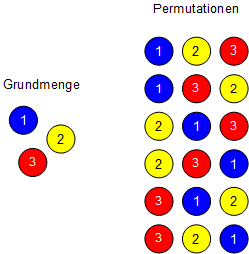
\includegraphics[width=0.5\textwidth]{Kapitel2/Bilder/image2}}
  \caption{Permutationen von drei verschiedenfarbigen Kugeln}
  \label{fig:Permutationen}
\end{figure}

\noindent Für das Beispiel ergibt sich mit N = 3 

\begin{equation}\label{eq:twotwentyfour}
M=N!=3\cdot 2\cdot 1=6
\end{equation}

\noindent Das Ergebnis deckt sich mit dem grafischen Ergebnis in Bild \ref{fig:Permutationen}.

\noindent Sind die N Elemente nicht alle verschieden, sondern lassen sie sich in K Klassen gleicher Elemente mit der jeweiligen Anzahl $N_{1}$, $N_{2}$, ..., $N_{K}$ einteilen, berechnet sich die Anzahl M unterscheidbarer Permutationen zu

\begin{equation}\label{eq:twotwentyfive}
M=\dfrac{N!}{\prod _{k=1}^{K}N_{\displaystyle k} ! } =\dfrac{N!}{N_{\displaystyle 1} !\cdot ...\cdot N_{k} !\cdot ...\cdot N_{K} !} 
\end{equation}

\noindent Die Division durch die Faktoren $N_{k}$! ergibt sich daraus, dass zwischen den Permutationen identischer Elemente innerhalb einer Klasse nicht unterschieden werden kann.\bigskip

\noindent
\colorbox{lightgray}{%
\arrayrulecolor{white}%
\renewcommand\arraystretch{0.6}%
\begin{tabular}{ wl{16.5cm} }
{\fontfamily{phv}\selectfont
\noindent{Beispiel: Permutationen bei zwei gelben und einer roten Kugel}}
\end{tabular}%
}\bigskip

\noindent Als Beispiel wird berechnet, wie viele Permutationen bei einer Gruppe von zwei gelben und einer roten Kugel entstehen k\"{o}nnen. Als Grundmenge stehen die Kugeln 1 - 3 zur Verf\"{u}gung. Die Kugel 1 ist rot, die Kugeln 2 und 3 sind gelb.

\noindent 
\begin{figure}[H]
  \centerline{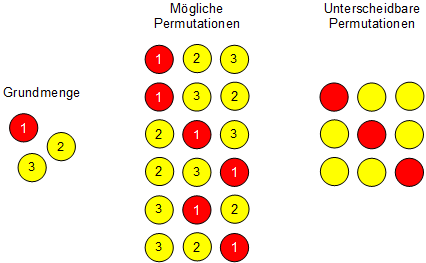
\includegraphics[width=0.5\textwidth]{Kapitel2/Bilder/image3}}
  \caption{Permutationen von zwei blauen und einer roten Kugel}
  \label{fig:Permutationen2}
\end{figure}

\noindent Es liegen N = 3 Kugeln vor, die in K = 2 Klassen aufgeteilt sind. In der Klasse 1 befinden sich $N_{1}$ = 2 gelbe Kugeln, in der Klasse 2 befindet sich $N_{2}$ = 1 rote Kugel. Damit berechnet sich die Anzahl M unterscheidbarer Permutationen aus 

\begin{equation}\label{eq:twotwentysix}
M=\dfrac{N!}{N_{\displaystyle k} !\cdot N_{\displaystyle k-1} !\cdot ...\cdot N_{\displaystyle 1} !} =\dfrac{3!}{2!\cdot 1!} =3
\end{equation}

\noindent Die Anzahl stimmt mit dem grafischen Ergebnis aus Bild \ref{fig:Permutationen2} \"{u}berein. \newline

\noindent Bei Permutationen werden alle Elemente einer Grundmenge angeordnet. Im Gegensatz dazu werden bei Variationen und Kombinationen nur Teile einer Grundmenge angeordnet.

\clearpage

\subsubsection{Variationen}
\noindent Wird aus einer Menge von N Elementen eine Teilmenge von K Elementen herausgegriffen und ist die Reihenfolge dieser Teilmenge von Bedeutung, so wird diese Zusammenstellung als Variation K-ter Ordnung bezeichnet. Es werden Variationen mit und ohne Wiederholung unterschieden.\newline

\noindent Bei Variationen ohne Wiederholung stehen bei der ersten Ziehung noch alle N Elemente zur Verf\"{u}gung. Bei der zweiten Ziehung ist ein Element bereits gezogen worden, es stehen nur noch (N - 1) Elemente zur Verf\"{u}gung. F\"{u}r N gegebene, voneinander verschiedene Elemente ergibt sich ohne Wiederholung die Anzahl M der Variationen K-ter Ordnung aus 

\begin{equation}\label{eq:twotwentyseven}
M=N\cdot (N-1)\cdot (N-2)\cdot ...\cdot (N-K+1)=\dfrac{N!}{(N-K)!}
\end{equation}

\noindent Werden N unbeschr\"{a}nkt oft wiederholbare verschiedene Elemente in Variationen K-ter Ordnung angeordnet, so existieren f\"{u}r jeden der K Pl\"{a}tze N M\"{o}glichkeiten. F\"{u}r Variationen mit Wiederholung ergibt sich damit eine Anzahl von M M\"{o}glichkeiten mit

\begin{equation}\label{eq:twotwentyeight}
M=N^{K}
\end{equation}

\noindent
\colorbox{lightgray}{%
\arrayrulecolor{white}%
\renewcommand\arraystretch{0.6}%
\begin{tabular}{ wl{16.5cm} }
{\fontfamily{phv}\selectfont
\noindent{Beispiel: Variationen bei verschiedenfarbigen Kugeln ohne und mit Wiederholung}}
\end{tabular}%
}\bigskip

\noindent Als Beispiel wird berechnet, wie viele Variationen sich bei einer Gruppe von einer roten, einer blauen und einer gelben Kugel entstehen k\"{o}nnen, von denen zwei Kugeln gezogen werden.

\noindent 
\begin{figure}[H]
  \centerline{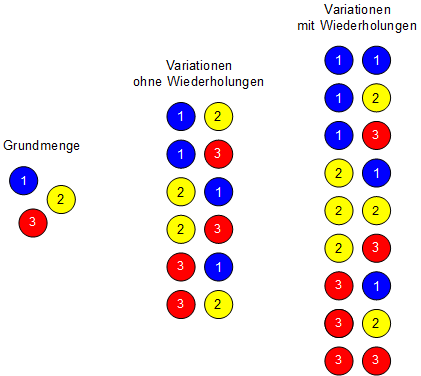
\includegraphics[width=0.5\textwidth]{Kapitel2/Bilder/image4}}
  \caption{Variationen von zwei Kugeln aus einer Grundmenge von drei unterschiedlichen Kugeln ohne und mit Wiederholung}
  \label{fig:Variationen}
\end{figure}

\noindent Die Berechnungen ergeben mit N = 3 und K = 2 die Anzahl der unterscheidbaren Variationen ohne Wiederholung zu

\begin{equation}\label{eq:twotwentynine}
M=\dfrac{3!}{(3-2)!} =6
\end{equation}

\noindent und mit Wiederholungen zu

\begin{equation}\label{eq:twothirty}
M=3^{2} =9
\end{equation}

\noindent Die Ergebnisse decken sich mit der grafischen L\"{o}sung in Bild \ref{fig:Variationen}

\subsubsection{Kombinationen}

\noindent Bei einer Kombination von Elementen bleibt die Reihenfolge unber\"{u}cksichtigt. Wie bei Variationen werden Anwendungen mit und ohne Wiederholung unterschieden. F\"{u}r Zufallsexperimente ohne Wiederholung wird die Anzahl von m\"{o}glichen Variationen in Gleichung \eqref{eq:twotwentyseven} berechnet. Dabei ergibt sich f\"{u}r jede Kombination eine Anzahl von K! Permutationen, die sich nur in der Reihenfolge der Anordnung unterscheiden. Ist die Anordnung der Elemente nicht von Bedeutung, so fallen von den Kombinationen diejenigen zusammen, die die gleichen Elemente in der Anordnung haben. Gem\"{a}{\ss} Gleichung \eqref{eq:twotwentythree} sind das bei einer Kombination K-ter Ordnung K! Elemente. Die Anzahl M von Kombinationen K-ter Ordnung aus einer Grundmenge mit N verschiedenen Elementen ohne Wiederholung betr\"{a}gt damit 

\begin{equation}\label{eq:twothirtyone}
M=(\begin{array}{c} {N} \\ {K} \end{array})=\dfrac{N\cdot (N-1)\cdot (N-2)\cdot ...\cdot (N-K+1)}{K!} =\dfrac{N!}{K!\cdot (N-K)!}
\end{equation}

\noindent Der Rechenausdruck in Gleichung \eqref{eq:twothirtyone} wird als N \"{u}ber K oder als Binomialkoeffizient bezeichnet. Die Anzahl M von Kombinationen K-ter Ordnung aus einer Grundmenge mit N verschiedenen Elementen mit Wiederholung kann auf eine \"{a}hnliche Art dargestellt werden. Es ergibt sich\bigskip

\begin{equation}\label{eq:twothirtytwo}
M=(\begin{array}{c} {N+K-1} \\ {K} \end{array})=\dfrac{(N+K-1)!}{K!\cdot (N-1)!}
\end{equation}

\noindent
\colorbox{lightgray}{%
\arrayrulecolor{white}%
\renewcommand\arraystretch{0.6}%
\begin{tabular}{ wl{16.5cm} }
{\fontfamily{phv}\selectfont
\noindent{Beispiel: Kombinationen bei verschiedenfarbigen Kugeln ohne und mit Wiederholung}}
\end{tabular}%
}\bigskip

\noindent Als Beispiel wird berechnet, wie viele Kombinationen sich bei einer Gruppe von einer roten, einer blauen und einer gelben Kugel ergeben k\"{o}nnen, von denen zwei Kugeln gezogen werden. Mit N = 3 und K = 2 ergibt sich die Anzahl der unterscheidbaren Kombinationen ohne Wiederholung zu 

\begin{equation}\label{eq:twothirtythree}
M=\dfrac{3!}{2!\cdot (3-2)!} =3
\end{equation}

\noindent und mit Wiederholungen ergibt sich 

\begin{equation}\label{eq:twothirtyfour}
M=(\begin{array}{c}{3+2-1}\\ {2} \end{array})=\dfrac{4!}{2!\cdot 2!} =6
\end{equation}

\noindent Die Ergebnisse decken sich mit der grafischen Lösung in Bild \ref{fig:Kombinationen}.

\noindent 
\begin{figure}[H]
  \centerline{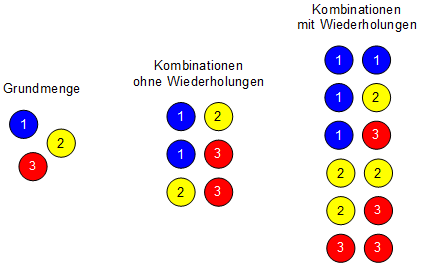
\includegraphics[width=0.7\textwidth]{Kapitel2/Bilder/image5}}
  \caption{Kombinationen von zwei Kugeln aus einer Grundmenge von drei unterschiedlichen Kugeln ohne und mit Wiederholung}
  \label{fig:Kombinationen}
\end{figure}

\noindent
\colorbox{lightgray}{%
\arrayrulecolor{white}%
\renewcommand\arraystretch{0.6}%
\begin{tabular}{ wl{16.5cm} }
{\fontfamily{phv}\selectfont
\noindent{Beispiel: Zahlenlotto}}
\end{tabular}%
}\bigskip

\noindent Bekanntestes Beispiel f\"{u}r die Berechnung von Kombinationsm\"{o}glichkeiten ist das Zahlenlotto, bei dem 6 Kugeln aus einer Menge aus 49 Kugeln gezogen werden. Die Kugeln k\"{o}nnen nicht mehrfach gezogen werden, die Reihenfolge der Ziehung ist nicht relevant. Es handelt sich um eine Kombination ohne Wiederholung und ohne Ber\"{u}cksichtigung der Reihenfolge. Die Anzahl von M\"{o}glichkeiten errechnet sich nach Gleichung \eqref{eq:twothirtyfive} zu

\begin{equation}\label{eq:twothirtyfive}
M=(\begin{array}{c} {49} \\ {6} \end{array})=\dfrac{49!}{6!\cdot 43!} \approx 14 Mio.
\end{equation}

\subsubsection{Überblick über Permutationen, Variationen und Kombinationen}

\noindent Bei der Berechnung von Permutationen, Variationen und Kombinationen m\"{u}ssen folgende Fragen beantwortet werden:


\begin{itemize}
    \item Welchen Umfang N hat die Ausgangsmenge?
    \item Wie kann die Auswahlprozedur modelliert werden (Reihenfolge, Wiederholungen, {\dots})?
    \item Welchen Umfang K hat die Auswahl?
\end{itemize}

\noindent Ist die Reihenfolge bei der Auswahl nicht relevant, handelt es sich bei dem Auswahlprozess um eine Kombination. Ist die Reihenfolge des Auswahlprozesses relevant und wird nur ein Teil aller Elemente der Grundmenge angeordnet, handelt es sich um eine Variation von Elementen. Werden alle Elemente angeordnet und ist die Reihenfolge der Auswahl wesentlich, handelt es sich um eine Permutation von Elementen. Mit diesen Informationen kann der geeignete Berechnungsprozess ausgew\"{a}hlt werden.

\noindent 
\begin{figure}[H]
  \centerline{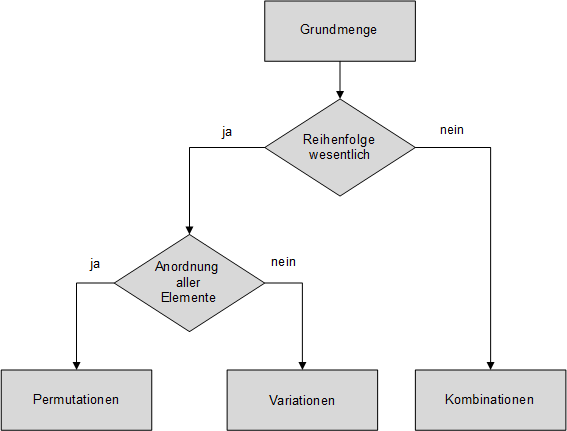
\includegraphics[width=0.9\textwidth]{Kapitel2/Bilder/image6}}
  \caption{Entscheidungsprozess für die verschiedenen Varianten der Kombinatorik}
  \label{fig:LandkarteKombinatorik}
\end{figure}

\clearpage

\noindent Tabelle \ref{tab:twotwo} fasst die Anzahl von Kombinationen und Variationen für die dargestellten Fälle mit und ohne Wiederholung zusammen. 

\begin{table}[H]
\setlength{\arrayrulewidth}{.1em}
\caption{Zusammenfassung der Berechnung von Permutationen, Kombinationen und Variationen}
\setlength{\fboxsep}{0pt}%
\colorbox{lightgray}{%
\arrayrulecolor{white}%
\begin{tabular}{| c | c |}
\hline
\parbox[c][0.28in][c]{3.3in}{\smallskip\centering\textbf{\fontfamily{phv}\selectfont{Variante der Kombinatorik}}} & 
\parbox[c][0.28in][c]{3.3in}{\smallskip\centering\textbf{\fontfamily{phv}\selectfont{Berechnungsgleichung}}}\\ \hline

\parbox[c][0.4in][c]{3.3in}{\centering{\fontfamily{phv}\selectfont{Permutation ohne Klassenbildung}}} &
\parbox[c][0.4in][c]{3.3in}{\centering{$M=N!$}}\\ \hline

\parbox[c][0.55in][c]{3.3in}{\centering{\fontfamily{phv}\selectfont{Permutation mit Klassenbildung}}} & 
\parbox[c][0.55in][c]{3.3in}{\centering{$M=\dfrac{N!}{\prod _{\displaystyle i=1}^{\displaystyle k}N_{\displaystyle i} ! } =\dfrac{N!}{N_{\displaystyle k} !\cdot N_{\displaystyle k-1} !\cdot ...\cdot N_{\displaystyle 1} !} $}}\\ \hline

\parbox[c][0.5in][c]{3.3in}{\centering{\fontfamily{phv}\selectfont{Variation ohne Wiederholung}}} & 
\parbox[c][0.5in][c]{3.3in}{\centering{$M=\dfrac{N!}{(N-K)!} $}}\\ \hline

\parbox[c][0.4in][c]{3.3in}{\centering{\fontfamily{phv}\selectfont{Variation mit Wiederholung}}} &
\parbox[c][0.4in][c]{3.3in}{\centering{$M=N^{K} $}}\\ \hline

\parbox[c][0.5in][c]{3.3in}{\centering{\fontfamily{phv}\selectfont{Kombinationohne Wiederholung}}} &
\parbox[c][0.5in][c]{3.3in}{\centering{$M=\left(\begin{array}{c} {N} \\ {K} \end{array}\right)=\dfrac{N!}{K!\cdot \left(N-K\right)!} $}}\\ \hline

\parbox[c][0.5in][c]{3.3in}{\centering{\fontfamily{phv}\selectfont{Kombinationohne Wiederholung}}} &
\parbox[c][0.5in][c]{3.3in}{\centering{$M=\left(\begin{array}{c} {N+K-1} \\ {K} \end{array}\right)=\dfrac{\left(M+K-1\right)!}{K!\cdot \left(N-1\right)!} $}}\\ \hline

\end{tabular}%
}
\label{tab:twotwo}
\end{table}

{\fontfamily{phv}\selectfont
\noindent\textbf{Befehle zur Berechnung in MATLAB}} \smallskip

\noindent Zur Berechnung der Anzahl von Permutationen, Kombinationen und Variationen werden im wesentlichen drei MATLAB-Befehle verwendet:

\begin{table}[H]
\setlength{\arrayrulewidth}{.1em}
\caption{MATLAB-Befehle zur Berechnung von Permutationen, Kombinationen und Variationen}
\setlength{\fboxsep}{0pt}%
\colorbox{lightgray}{%
\arrayrulecolor{white}%
\begin{tabular}{| c | c | c |}
\hline

\parbox[c][0.35in][c]{2.18in}{\centering{\fontfamily{phv}\selectfont\textbf{Fakultät}}} &
\parbox[c][0.35in][c]{2.18in}{\centering{$M=N!$}}&
\parbox[c][0.35in][c]{2.18in}{\centering{\fontfamily{phv}\selectfont{factorial(N)}}}\\ \hline

\parbox[c][0.35in][c]{2.18in}{\centering{\fontfamily{phv}\selectfont\textbf{Potenz}}} &
\parbox[c][0.35in][c]{2.18in}{\centering{$M=N^{K}$}}&
\parbox[c][0.35in][c]{2.18in}{\centering{\fontfamily{phv}\selectfont{N$\mathrm{\wedge}$K}}}\\ \hline

\parbox[c][0.5in][c]{2.18in}{\centering{\fontfamily{phv}\selectfont\textbf{Binomialkoeffizient}}} &
\parbox[c][0.5in][c]{2.18in}{\centering{$M=\left(\begin{array}{c} {N} \\ {K} \end{array}\right)=\dfrac{N!}{K!\cdot \left(N-K\right)!}$}}&
\parbox[c][0.5in][c]{2.18in}{\centering{\fontfamily{phv}\selectfont{nchoosek(N,K)}}}\\ \hline

\end{tabular}%
}
\label{tab:twothree}
\end{table}

{\fontfamily{phv}\selectfont
\noindent\textbf{Befehle zur Berechnung in Python}} \smallskip

\noindent Zur Berechnung der Anzahl von Permutationen, Kombinationen und Variationen werden im wesentlichen drei Python-Befehle verwendet:

\begin{table}[H]
\setlength{\arrayrulewidth}{.1em}
\caption{Python-Befehle zur Berechnung von Permutationen, Kombinationen und Variationen}
\setlength{\fboxsep}{0pt}%
\colorbox{lightgray}{%
\arrayrulecolor{white}%
\begin{tabular}{| c | c | c |}
\hline

\parbox[c][0.35in][c]{2.18in}{\centering{\fontfamily{phv}\selectfont\textbf{Fakultät}}} &
\parbox[c][0.35in][c]{2.18in}{\centering{$M=N!$}}&
\parbox[c][0.35in][c]{2.18in}{\centering{\fontfamily{phv}\selectfont{scipy.special.factorial}}}\\ \hline

\parbox[c][0.35in][c]{2.18in}{\centering{\fontfamily{phv}\selectfont\textbf{Potenz}}} &
\parbox[c][0.35in][c]{2.18in}{\centering{$M=N^{K}$}}&
\parbox[c][0.35in][c]{2.18in}{\centering{\fontfamily{phv}\selectfont{scipy.special.factorial}}}\\ \hline

\parbox[c][0.5in][c]{2.18in}{\centering{\fontfamily{phv}\selectfont\textbf{Binomialkoeffizient}}} &
\parbox[c][0.5in][c]{2.18in}{\centering{$M=\left(\begin{array}{c} {N} \\ {K} \end{array}\right)=\dfrac{N!}{K!\cdot \left(N-K\right)!}$}}&
\parbox[c][0.5in][c]{2.18in}{\centering{\fontfamily{phv}\selectfont{scipy.special.comb}}}\\ \hline

\end{tabular}%
}
\label{tab:twofour}
\end{table}

\noindent Mit den berechneten Werten lassen sich die Anzahl möglicher Ereignisse und die Anzahl günsti-ger Ereignisse bestimmen. Mit den Ergebnissen wird die Wahrscheinlichkeit für das entspre-chende Ereignis berechnet. 

\subsection{Aufbau von Ereignisbäumen}

\noindent Oftmals k\"{o}nnen Zufallsprozesse aus mehreren nacheinander ablaufenden Zufallsexperimenten modelliert werden. In dem Fall handelt es sich um ein sogenanntes mehrstufiges Zufallsexperiment. Ein anschauliches, grafisches Hilfsmittel bei der Berechnung von Wahrscheinlichkeiten solcher mehrstufigen Zufallsexperimente ist der Ereignisbaum [Papu01][Papu01]. Er besteht aus einer Wurzel, dem Ausgangspunkt der Zufallsexperimente, mehreren Verzweigungspunkten und einer Vielzahl von Zweigen.

\noindent 
\begin{figure}[H]
  \centerline{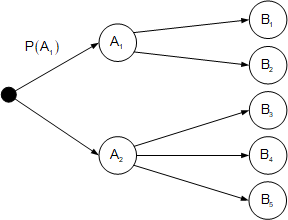
\includegraphics[width=0.5\textwidth]{Kapitel2/Bilder/image7}}
  \caption{Darstellung eines Ereignisbaumes}
  \label{fig:DarstellungEreignisbaum}
\end{figure}

\noindent In Bild \ref{fig:DarstellungEreignisbaum} ist der prinzipielle Aufbau eines zweistufigen Ereignisbaumes zu erkennen. Der Ausgangspunkt des Zufallsexperiments, die Wurzel, wird durch einen schwarzen Punkt dargestellt. Die Verzweigungspunkte $A_{1}$ und $A_{2}$ charakterisieren die m\"{o}glichen Ereignisse f\"{u}r das erste Zufallsexperiment. Die von diesen Verzweigungspunkten ausgehenden Zweige f\"{u}hren zu den jeweils m\"{o}glichen Ergebnissen der folgenden 2. Stufe, die durch $B_{1}$ bis $B_{5}$ bezeichnet sind.\newline

\noindent Die \"{U}bergangswahrscheinlichkeit von einem Ereignis zu einem Folgeereignis wird an den betreffenden Zweig geschrieben. So gibt P($A_{1}$) an, mit welcher Wahrscheinlichkeit das Ereignis $A_{1}$ eintritt. Ein m\"{o}gliches Endergebnis des Zufallsprozesses wird dann immer von der Wurzel ausgehend l\"{a}ngs eines Pfades erreicht. Dieser besteht meist aus mehreren Zweigen. Die Berechnung der Wahrscheinlichkeit eines bestimmten Endergebnisses erfolgt unter Anwendung folgender Rechenregeln:

\begin{itemize}
    \item Wahrscheinlichkeiten entlang eines Pfades werden multipliziert
    \item Führen mehrere Pfade zum gleichen Endergebnis, so addieren sich ihre Wahrscheinlichkeiten
\end{itemize}

\noindent
\colorbox{lightgray}{%
\arrayrulecolor{white}%
\renewcommand\arraystretch{0.6}%
\begin{tabular}{ wl{16.5cm} }
{\fontfamily{phv}\selectfont
\noindent{Beispiel: Ereignisbaum für das zweimalige Würfeln}}
\end{tabular}%
}\bigskip

\noindent Um den Umgang mit Ereignisb\"{a}umen zu verdeutlichen, wird das zweimalige W\"{u}rfeln eines regelm\"{a}{\ss}igen W\"{u}rfels betrachtet. Es handelt sich dabei um ein zweistufiges Zufallsexperiment. F\"{u}r das W\"{u}rfeln mit einem W\"{u}rfel k\"{o}nnen eine Menge der geraden Zahlen und eine Menge der ungeraden Zahlen definiert werden. Beide Mengen sind disjunkt, zusammen stellen sie das sichere Ereignis dar, weil jede gew\"{u}rfelte Augenzahl entweder gerade oder ungerade ist.

\noindent Als Beispiel wird die Wahrscheinlichkeit daf\"{u}r ausgerechnet, dass bei zwei W\"{u}rfen mit einem regelm\"{a}{\ss}igen W\"{u}rfel eine gerade Augensumme erzielt wird. Dieses Ereignis wird als B bezeichnet. Es ergibt sich der in Bild \ref{fig:EinfuehrungsbeispielEreignisbaum} dargestellte Ereignisbaum.

\noindent 
\begin{figure}[H]
  \centerline{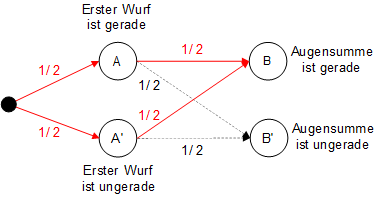
\includegraphics[width=0.5\textwidth]{Kapitel2/Bilder/image8}}
  \caption{Darstellung eines Ereignisbaumes f\"{u}r das zweimalige W\"{u}rfeln}
  \label{fig:EinfuehrungsbeispielEreignisbaum}
\end{figure}

\noindent Die gerade Augensumme kann sich auf zweierlei Arten ergeben, da beim ersten Wurf entweder eine gerade oder eine ungerade Augenzahl gew\"{u}rfelt werden kann. Wird beim ersten Wurf eine gerade Zahl gew\"{u}rfelt, muss auch beim zweiten Wurf eine gerade Zahl gew\"{u}rfelt werden. Wird beim ersten Wurf eine ungerade Zahl gew\"{u}rfelt, muss auch beim zweiten Wurf eine ungerade Zahl gew\"{u}rfelt werden. Die Gesamtwahrscheinlichkeit ergibt sich aus der Summe der Wahrscheinlichkeiten dieser beiden Pfade.

\begin{equation}\label{eq:twothirtysix}
P(B)=\dfrac{1}{2} \cdot \dfrac{1}{2} +\dfrac{1}{2} \cdot \dfrac{1}{2} =\dfrac{1}{2}
\end{equation}

\clearpage

\subsection{Wahrscheinlichkeitsbegriff der Statistik nach Kolmogoroff}

\noindent Die klassische Wahrscheinlichkeitsrechnung nach Laplace beruht darauf, den Begriff der Wahrscheinlichkeit auf die Gleichwahrscheinlichkeit von Elementarereignissen zur\"{u}ckzuf\"{u}hren. Ereignismengen werden mit den vorgestellten Mengenoperationen auf Elementarereignisse zur\"{u}ckgef\"{u}hrt. Es existieren aber auch Zufallsexperimente, bei denen der Ereignisraum unendlich viele Elementarereignisse aufweist. Ein Ereignis wird damit ein stetiges Kontinuum. Soll zum Beispiel die Toleranzverteilung bei der Fertigung von Passstiften analysiert werden, ist der Ereignisraum kontinuierlich. Der Wahrscheinlichkeitsbegriff von Laplace kann deshalb nicht angewendet werden. Aus diesem Grund hat Kolmogoroff ihn verallgemeinert.\newline

\noindent Der statistische Begriff der Wahrscheinlichkeit nach Kolmogoroff beruht auf Axiomen. Ein Axiom ist eine grundlegende Aussage, die zu anderen Axiomen widerspruchsfrei ist. Aus Axiomen lassen sich alle sonstigen S\"{a}tze des Systems logisch ableiten. Den Ausgangspunkt f\"{u}r den Wahrscheinlichkeitsbegriff der Statistik nach Kolmogoroff bildet die Erfahrung, dass das Eintreffen von Ereignissen bei den meisten Zufallsprozessen bei vielfacher Wiederholung einer gewissen Gesetzm\"{a}{\ss}igkeit unterliegt. Insbesondere erweist sich die relative H\"{a}ufigkeit eines Experimentes f\"{u}r gro{\ss}e Stichprobenumf\"{a}nge als stabil. Diese ist definiert als Quotient aus der absoluten H\"{a}ufigkeit, mit der ein Wert vorliegt, und dem Stichprobenumfang N.

\begin{equation}\label{eq:twothirtyseven}
h(A)=\dfrac{h_{A} (A)}{N}
\end{equation}

\noindent Bild \ref{fig:RelativeHaeufigkeitBeimWuerfeln} zeigt f\"{u}r ein W\"{u}rfelexperiment mit einem regelm\"{a}{\ss}igen W\"{u}rfel die relative H\"{a}ufigkeit, eine gerade Zahl zu w\"{u}rfeln.

\noindent 
\begin{figure}[H]
  \centerline{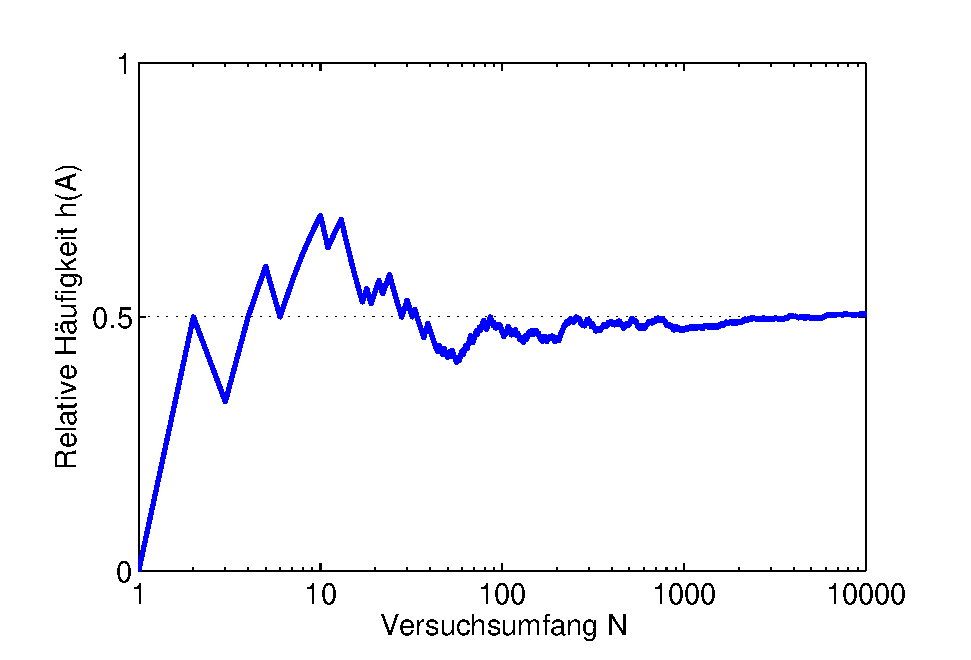
\includegraphics[width=0.5\textwidth]{Kapitel2/Bilder/image9}}
  \caption{Relative H\"{a}ufigkeit mit einem regelm\"{a}{\ss}igen W\"{u}rfel eine gerade Zahl zu w\"{u}rfeln als Funktion der Anzahl von Versuchen}
  \label{fig:RelativeHaeufigkeitBeimWuerfeln}
\end{figure}

\noindent Sind die relativen H\"{a}ufigkeiten der Ereignisse bei einem Experiment nahezu konstant, weist das Experiment eine statistische Regelm\"{a}{\ss}igkeit oder Stabilit\"{a}t der relativen H\"{a}ufigkeit auf. Die meisten praktischen Zufallsexperimente haben diese Stabilit\"{a}tseigenschaft. Trifft bei wiederholtem Ausf\"{u}hren eines Experimentes das Ereignis A mit der relativen H\"{a}ufigkeit h(A) ein, so wird die relative H\"{a}ufigkeit als die Wahrscheinlichkeit P(A) f\"{u}r das Ereignis A definiert. Die Wahrscheinlichkeit P(A) ist damit das theoretische Gegenst\"{u}ck zu der empirischen relativen H\"{a}ufigkeit h(A), auf die in Kapitel 3 eingegangen wird.
\clearpage
\subsubsection{Axiome der Wahrscheinlichkeitsrechnung nach Kolmogoroff}

\noindent Für die Wahrscheinlichkeit P(A) gelten nach Kolmogoroff folgende Axiome:\bigskip

{\fontfamily{phv}\selectfont
\noindent\textbf{Axiom 1}} \smallskip

\noindent Die Wahrscheinlichkeit P(A) eines Ereignisses A bei einem Experiment ist eine eindeutig be-stimmte reelle, nicht negative Zahl, die höchstens gleich 1 ist.

\begin{equation}\label{eq:twothirtyeight}
0\le P(A)\le 1
\end{equation}

\noindent Dieses Axiom wird von dem Wahrscheinlichkeitsbegriff nach Laplace erf\"{u}llt. Die Anzahl der g\"{u}nstigen F\"{a}lle eines Experimentes ist stets kleiner oder gleich der Anzahl der m\"{o}glichen F\"{a}lle.\bigskip

{\fontfamily{phv}\selectfont
\noindent\textbf{Axiom 2}} \smallskip

\noindent Ein sicheres Ereignis S bei einem Experiment hat die Wahrscheinlichkeit 1.

\begin{equation}\label{eq:twothirtynine}
P(S)=1
\end{equation}

\noindent Sind zwei Ereignisse B und C \"{a}quivalent, so sind ihre Wahrscheinlichkeiten gleich gro{\ss}.

\begin{equation}\label{eq:twofourty}
P(B)=P(C)
\end{equation}

\noindent Auch dieses Axiom wird von der Laplaceschen Definition der Wahrscheinlichkeit erf\"{u}llt. Im Fall des sicheren Ereignisses S entspricht die Anzahl der g\"{u}nstigen F\"{a}lle gerade der Anzahl der m\"{o}glichen F\"{a}lle, sodass sich als Wahrscheinlichkeit der Wert 1 ergibt. Sind zwei Ereignisse identisch, so ist die Anzahl der g\"{u}nstigen F\"{a}lle gleich gro{\ss} und in beiden F\"{a}llen ergibt sich die gleiche Wahrscheinlichkeit.\bigskip

{\fontfamily{phv}\selectfont
\noindent\textbf{Axiom 3}} \smallskip

\noindent Schlie{\ss}en sich zwei Ereignisse A und B bei einem Experiment gegenseitig aus, so gilt bei dem Experiment

\begin{equation}\label{eq:twofourtyone}
P(A\cup B)=P(A)+P(B)
\end{equation}

\noindent
\colorbox{lightgray}{%
\arrayrulecolor{white}%
\renewcommand\arraystretch{0.6}%
\begin{tabular}{ wl{16.5cm} }
{\fontfamily{phv}\selectfont
\noindent{Beispiel: Würfelexperiment und Axiome nach Kolmogoroff}}
\end{tabular}%
}\bigskip

\noindent Das erste Axiom ist f\"{u}r das W\"{u}rfelexperiment erf\"{u}llt. Die Anzahl der g\"{u}nstigen F\"{a}lle des W\"{u}rfelexperimentes A ist stets kleiner oder gleich der Anzahl der m\"{o}glichen F\"{a}lle. Damit liegt die Wahrscheinlichkeit P(A) in dem Bereich 0 $\leq$ P(A) $\leq$ 1.\newline

\noindent Sind alle Ereignisse beim W\"{u}rfeln g\"{u}nstig, ergibt sich das sichere Ereignis S. Die Anzahl g\"{u}nstiger F\"{a}lle entspricht der Anzahl m\"{o}glicher F\"{a}lle und die Wahrscheinlichkeit ist P(S) = 1. \newline

\noindent Auch das dritte Axiom kann an dem W\"{u}rfelexperiment mit einem W\"{u}rfel verdeutlicht werden. Das W\"{u}rfeln der Zahlen 1 und 2 schlie{\ss}t sich gegenseitig aus. Die Wahrscheinlichkeit f\"{u}r einen Wurf mit der Augenzahl 1 oder 2 entspricht der Vereinigungsmenge A $\cup$ B. Die klassische Wahrscheinlichkeit ergibt sich aus der Summe der Wahrscheinlichkeit f\"{u}r den Wurf einer 1 und der einer 2.

\subsubsection{S\"{a}tze zur Wahrscheinlichkeitsrechnung nach Kolmogoroff}

\noindent Auf Basis dieser drei Axiome zur Wahrscheinlichkeit lassen sich weitere S\"{a}tze ableiten, die im Folgenden dargestellt werden.\bigskip

{\fontfamily{phv}\selectfont
\noindent\textbf{Additionssatz der Wahrscheinlichkeit f\"{u}r komplement\"{a}re Ereignisse}} \smallskip

\noindent Ein Ereignis, das genau dann eintrifft, wenn das Ereignis A nicht eintrifft, wird als komplement\"{a}res Ereignis A' bezeichnet. Da entweder das Ereignis A oder das komplement\"{a}re Ereignis A' eintrifft, gilt

\begin{equation}\label{eq:twofourtytwo}
P(A\cup A')=P(S)=1
\end{equation}

\noindent Gem\"{a}{\ss} Axiom 3 gilt

\begin{equation}\label{eq:twofourtythree}
P(A)+P(A')=1
\end{equation}

\noindent oder

\begin{equation}\label{eq:twofourtyfour}
P(A')=1-P(A)
\end{equation}

\noindent Aus diesem Satz folgt f\"{u}r die Wahrscheinlichkeit f\"{u}r ein unm\"{o}gliches Ereignis U 

\begin{equation}\label{eq:twofourtyfive}
P(U)=1-P(S)=1-1=0
\end{equation}

\noindent
\colorbox{lightgray}{%
\arrayrulecolor{white}%
\renewcommand\arraystretch{0.6}%
\begin{tabular}{ wl{16.5cm} }
{\fontfamily{phv}\selectfont
\noindent{Beispiel: Würfelexperiment und Additionssatz für komplement\"{a}re Ereignisse}}
\end{tabular}%
}\bigskip

\noindent Zum Beispiel berechnet sich die Wahrscheinlichkeit des Ereignisses D, beim W\"{u}rfeln eine 4 zu erzielen, aus

\begin{equation}\label{eq:twofourtysix}
P\left(D\right)=\dfrac{1}{6}
\end{equation}

\noindent Die Wahrscheinlichkeit D', keine 4 zu erzielen, ergibt sich entsprechend zu 

\begin{equation}\label{eq:twofourtyseven}
P\left(D'\right)=1-\dfrac{1}{6} =\dfrac{5}{6}
\end{equation}

{\fontfamily{phv}\selectfont
\noindent\textbf{Additionssatz der Wahrscheinlichkeit f\"{u}r mehrere sich ausschlie{\ss}ende Ereignisse}} \smallskip

\noindent Sind $A_{1}$, $A_{2}$, ..., $A_{N}$ abz\"{a}hlbar unendlich viele Ereignisse, die sich bei einem Experiment gegenseitig ausschlie{\ss}en, so gilt bei diesem Experiment

\begin{equation}\label{eq:twofourtyeight}
P(\bigcup _{n=1}^{N}A_{n})=P(A_{1} \cup A_{2} \cup ...\cup A_{N} )=P(A_{1})+P(A_{2})+...+P(A_{N})=\sum _{n=1}^{N}P(A_{n})
\end{equation}

\noindent Dieser Additionssatz f\"{u}r beliebig viele Ereignisse, die sich gegenseitig ausschlie{\ss}en, kann durch wiederholte Anwendung von Axiom 3 der statistischen Wahrscheinlichkeit hergeleitet werden. 

{\fontfamily{phv}\selectfont
\noindent\textbf{Additionssatz der Wahrscheinlichkeit für beliebige Ereignisse}} \smallskip

\noindent Schlie{\ss}en sich die Ereignisse A und B eines Zufallsexperimentes nicht gegenseitig aus und haben sie die Wahrscheinlichkeiten P(A) und P(B), so gilt für die Wahrscheinlichkeit f\"{u}r das Ereignis $A \cup B$ 

\begin{equation}\label{eq:twofourtynine}
P(A\cup B)=P(A)+P(B)-P(A\cap B)
\end{equation}

\noindent Zum Beweis des Satzes wird wird die Vereinigungsmenge in zwei unabh\"{a}ngige Mengen zerlegt.

\begin{equation}\label{eq:twofifty}
P\left(A\cup B\right)=P\left(A\cup \left(A'\cap B\right)\right)
\end{equation}

\noindent Mit Axiom 3 der Wahrscheinlichkeit nach Kolmogoroff folgt 

\begin{equation}\label{eq:twofiftyone}
P\left(A\cup B\right)=P\left(A\right)+P\left(A'\cap B\right)
\end{equation}

\noindent Addition und Subtraktion des Ausdrucks $P(A\cap B)$ f\"{u}hrt zu

\begin{equation}\label{eq:twofiftytwo}
\begin{split}
P(A\cup B) & = P(A)+P(A'\cap B)+P(A\cap B)-P(A\cap B) \\ 
& = P(A)+(P(A'\cap B)+P(A\cap B))-P(A\cap B)\\ 
& = P(A)+P(B)-P(A\cap B)
\end{split}
\end{equation}

\noindent
\colorbox{lightgray}{%
\arrayrulecolor{white}%
\renewcommand\arraystretch{0.6}%
\begin{tabular}{ wl{16.5cm} }
{\fontfamily{phv}\selectfont
\noindent{Beispiel: Würfelexperiment und Additionssatz für beliebige Ereignisse}}
\end{tabular}%
}\bigskip

\noindent Anschaulich kann die Wahrscheinlichkeit wie bereits bei dem Laplaceschen Begriff der Wahrscheinlichkeit erkl\"{a}rt werden.

\noindent 
\begin{figure}[H]
  \centerline{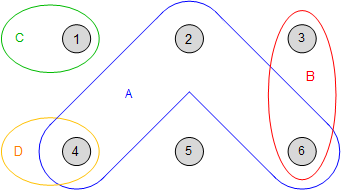
\includegraphics[width=0.5\textwidth]{Kapitel2/Bilder/image10}}
  \caption{Darstellung des Zufallsexperimentes Würfeln mit einem regelmäßigem Würfel}
  \label{fig:Mengen1}
\end{figure}

\noindent F\"{u}r das Beispiel ergibt sich die Wahrscheinlichkeit f\"{u}r das Ereignis $A \cup B$ aus

\begin{equation}\label{eq:twofiftythree}
P(A\cup B)=P(A)+P(B)-P(A\cap B)=\dfrac{1}{2} +\dfrac{1}{3} -\dfrac{1}{6} =\dfrac{2}{3}
\end{equation}

\noindent Das Ergebnis kann dadurch verifiziert werden, dass die Wahrscheinlichkeiten der W\"{u}rfe mit den Augenzahlen 2, 3, 4 und 6 addiert werden. Das Subtrahieren der Wahrscheinlichkeit P(A $\cap$ B) in Gleichung \eqref{eq:twofiftythree} ist notwendig, damit die Wahrscheinlichkeit des Wurfes mit der Augenzahl 6 nicht doppelt in das Ergebnis eingeht.\bigskip

{\fontfamily{phv}\selectfont
\noindent\textbf{Bedingte Wahrscheinlichkeit}} \smallskip

\noindent Sind A und B Ereignisse und ist bei einem Experiment $P(A) \neq 0$, so wird mit der Schreibweise $P(B|A)$ die Wahrscheinlichkeit des Ereignisses B unter der Voraussetzung oder Hypothese verstanden, dass das Ereignis A bereits eingetroffen ist. $P(B|A)$ wird auch als die bedingte Wahrscheinlichkeit des Ereignisses B unter der Hypothese A bezeichnet. Sie berechnet sich aus

\begin{equation}\label{eq:twofiftyfour}
P(B|A)=\dfrac{P(A\cap B)}{P(A)}
\end{equation}

\noindent
\colorbox{lightgray}{%
\arrayrulecolor{white}%
\renewcommand\arraystretch{0.6}%
\begin{tabular}{ wl{16.5cm} }
{\fontfamily{phv}\selectfont
\noindent{Beispiel: Würfelexperiment}}
\end{tabular}%
}\bigskip

\noindent Als Beispiel f\"{u}r die Berechnung der bedingten Wahrscheinlichkeit wird wieder das W\"{u}rfelexperiment herangezogen. Das Ereignis A ist das W\"{u}rfeln einer geraden Zahl, das Ereignis $B_{2}$ ist das W\"{u}rfeln der Zahl 2. Gesucht ist die Wahrscheinlichkeit $P(B_{2}|A)$, also die Wahrscheinlichkeit f\"{u}r das W\"{u}rfeln der Zahl 2 unter der Bedingung, dass eine gerade Augenzahl gew\"{u}rfelt wurde.

\noindent Das Beispiel kann in Form eines Ereignisbaumes modelliert werden. Ausgehend von der Wurzel kann eine gerade oder eine ungerade Zahl gew\"{u}rfelt werden. Jedes dieser Zwischenergebnisse unterteilt sich in drei m\"{o}gliche Endergebnisse. Die Wahrscheinlichkeiten ergeben sich daher wie in Bild \ref{fig:Wuerfeln} dargestellt.

\noindent 
\begin{figure}[H]
  \centerline{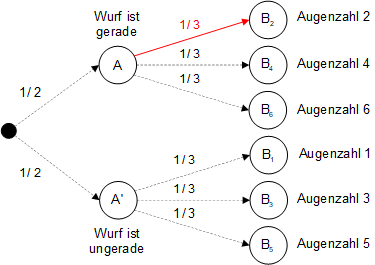
\includegraphics[width=0.5\textwidth]{Kapitel2/Bilder/image11}}
  \caption{Ereignisbaum zur Modellierung eines W\"{u}rfelexperiments}
  \label{fig:Wuerfeln}
\end{figure}

\noindent Die Wahrscheinlichkeit f\"{u}r eine gerade Augenzahl ergibt sich zu

\begin{equation}\label{eq:twofiftyfive}
P(A)=\dfrac{1}{2}
\end{equation}

\noindent Um die Wahrscheinlichkeit $P(A\cap B_{2})$ zu berechnen, werden die Wahrscheinlichkeiten des entsprechenden Pfades multipliziert

\begin{equation}\label{eq:twofiftysix}
P(A\cap B_{2} )=\dfrac{1}{2} \cdot \dfrac{1}{3} =\dfrac{1}{6}
\end{equation}

\noindent Damit berechnet sich die bedingte Wahrscheinlichkeit von

\begin{equation}\label{eq:twofiftyseven}
P(B_{2} |A)=\dfrac{P(A\cap B_{2})}{P(A)} =\dfrac{1/6}{1/2} =\dfrac{1}{3}
\end{equation}

\noindent Diese bedingte Wahrscheinlichkeit entspricht der \"{U}bergangswahrscheinlichkeit in dem Ereignisbaum. Sie kann direkt aus dem Ereignisbaum des Zufallsexperiments abgelesen werden. Unter der Annahme, dass eine gerade Zahl gew\"{u}rfelt wurde, kann direkt die bedingte Wahrscheinlichkeit $P(B_{2}|A)$ am rot eingezeichneten Zweig abgelesen werden.\bigskip

{\fontfamily{phv}\selectfont
\noindent\textbf{Multiplikationssatz der Wahrscheinlichkeit}} \smallskip

\noindent Nach Gleichung \eqref{eq:twofiftyfour} gilt f\"{u}r die bedingte Wahrscheinlichkeit 

\begin{equation}\label{eq:twofiftyeight}
P(B|A)=\dfrac{P(A\cap B)}{P(A)}
\end{equation}

\noindent und bei Tauschen der Variablen A und B 

\begin{equation}\label{eq:twofiftynine}
P(A|B)=\dfrac{P(A\cap B)}{P(B)}
\end{equation}

\noindent Damit kann die Wahrscheinlichkeit f\"{u}r die Schnittmenge P(A$\cap$B) angegeben werden. Haben zwei Ereignisse A und B bei einem Experiment die Wahrscheinlichkeit P(A) und P(B), so betr\"{a}gt die Wahrscheinlichkeit f\"{u}r gleichzeitiges Eintreffen von den Ereignissen A und B 

\begin{equation}\label{eq:twosixty}
P(A\cap B)=P(A|B)\cdot P(B)=P(B|A)\cdot P(A)
\end{equation}

\noindent
\colorbox{lightgray}{%
\arrayrulecolor{white}%
\renewcommand\arraystretch{0.6}%
\begin{tabular}{ wl{16.5cm} }
{\fontfamily{phv}\selectfont
\noindent{Beispiel: Würfelexperiment}}
\end{tabular}%
}\bigskip

\noindent Diese Aussagen lassen sich ebenfalls mit dem W\"{u}rfelexperiment veranschaulichen. Ein Ereignis A ist dadurch definiert, dass beim W\"{u}rfeln mit einem regelm\"{a}{\ss}igen W\"{u}rfel eine gerade Zahl gew\"{u}rfelt wird. Das Ereignis B ist dadurch definiert, dass eine durch 3 teilbare Zahl gew\"{u}rfelt wird. Damit ergibt sich die Wahrscheinlichkeit f\"{u}r die Schnittmenge aus beiden Aussagen zu 

\begin{equation}\label{eq:twosixtyone}
P(A\cap B)=P(A|B)\cdot P(B)=\dfrac{1}{2} \cdot \dfrac{2}{6} =\dfrac{1}{6}
\end{equation}

\noindent oder zu 

\begin{equation}\label{eq:twosixtytwo}
P(B\cap A)=P(B|A)\cdot P(A)=\dfrac{1}{3} \cdot \dfrac{1}{2} =\dfrac{1}{6}
\end{equation}

\noindent Beide Ergebnisse sind identisch und geben die Wahrscheinlichkeit an, mit der die Zahl 6 gew\"{u}rfelt wird, denn es ist das einzige Ereignis, das die Bedingungen A und B erf\"{u}llt.\bigskip

{\fontfamily{phv}\selectfont
\noindent\textbf{Statistische Unabhängigkeit von Ereignissen}} \smallskip

\noindent Ist das Eintreffen eines Ereignisses A von dem Eintreffen eines Ereignisses B unabh\"{a}ngig, so gilt

\begin{equation}\label{eq:twosixtythree}
P(A|B)=P(A)
\end{equation}

\noindent und

\begin{equation}\label{eq:twosixtyfour}
P(B|A)=P(B)
\end{equation}

\noindent Die Ereignisse A und B werden in diesem Fall auch als statistisch unabh\"{a}ngig bezeichnet. Durch Einsetzen vereinfacht sich Gleichung \eqref{eq:twosixty} f\"{u}r den Fall unabh\"{a}ngiger Variablen zu 

\begin{equation}\label{eq:twosixtyfive}
P(A\cap B)=P(A|B)\cdot P(B)=P(A)\cdot P(B)=P(B)\cdot P(A)=P(B|A)\cdot P(A)
\end{equation}

\noindent Die statistische Unabh\"{a}ngigkeit ist bei W\"{u}rfelexperimenten unmittelbar erkennbar. Bei komplexeren Vorg\"{a}ngen kann eine statistische Unabh\"{a}ngigkeit oft nicht so klar erkannt werden. Gleichung \eqref{eq:twosixtyfive} erm\"{o}glicht es, statistische Unabh\"{a}ngigkeit nachzuweisen. Der Begriff der statistischen Unabh\"{a}ngigkeit l\"{a}sst sich auch auf mehr als zwei unabh\"{a}ngige Variable erweitern.

\begin{equation}\label{eq:twosixtysix}
P\left(\bigcap _{n=1}^{N}A_{n}  \right)=\prod _{n=1}^{N}P\left(A_{n} \right)
\end{equation}

\noindent Diese Rechenregeln k\"{o}nnen als Test f\"{u}r die statistische Unabh\"{a}ngigkeit von Gr\"{o}{\ss}en verwendet werden. Im Fall der statistischen Unabh\"{a}ngigkeit muss die Bedingung

\begin{equation}\label{eq:twosixtyseven}
P(A\cap B)=P(A)\cdot P(B)=P(B)\cdot P(A)
\end{equation}

\noindent erf\"{u}llt sein.\bigskip

\noindent
\colorbox{lightgray}{%
\arrayrulecolor{white}%
\renewcommand\arraystretch{0.6}%
\begin{tabular}{ wl{16.5cm} }
{\fontfamily{phv}\selectfont
\noindent{Beispiel: Statistische Unabhängigkeit beim Würfelexperiment}}
\end{tabular}%
}\bigskip

\noindent Als Beispiel wird die Wahrscheinlichkeit berechnet, bei zweimaligem W\"{u}rfeln mit einem regelm\"{a}{\ss}igen W\"{u}rfel zwei Sechsen zu erhalten. Die Wahrscheinlichkeit, beim ersten Wurf eine 6 zu w\"{u}rfeln betr\"{a}gt 

\begin{equation}\label{eq:twosixtyeight}
P(A)=\dfrac{1}{6}
\end{equation}

\noindent Da der W\"{u}rfel nicht ver\"{a}ndert wird, ist die Ausgangssituation beim zweiten Wurf dieselbe wie beim ersten. Das Ergebnis des ersten Zuges hat also keinerlei Einfluss auf das Ergebnis des zweiten. Demnach handelt es sich um unabh\"{a}ngige Ereignisse. Die Wahrscheinlichkeit, beim zweiten Wurf eine 6 zu erhalten, betr\"{a}gt ebenfalls 

\begin{equation}\label{eq:twosixtynine}
P(B)=\dfrac{1}{6}
\end{equation}

\noindent Die Wahrscheinlichkeit f\"{u}r das zweimalige W\"{u}rfeln einer 6 betr\"{a}gt

\begin{equation}\label{eq:twoseventy}
P=\dfrac{1}{6} \cdot \dfrac{1}{6} =\dfrac{1}{36}
\end{equation}

\noindent Dasselbe Ergebnis ergibt sich bei der Berechnung der Gesamtwahrscheinlichkeit des Endergebnisses im Ereignisbaum.\bigskip

\noindent
\colorbox{lightgray}{%
\arrayrulecolor{white}%
\renewcommand\arraystretch{0.6}%
\begin{tabular}{ wl{16.5cm} }
{\fontfamily{phv}\selectfont
\noindent{Beispiel: Statistische Unabhängigkeit von Spezifikationsmerkmalen}}
\end{tabular}%
}\bigskip

\noindent Bei einer Untersuchung von Einspritzd\"{u}sen werden 100 Einspritzd\"{u}sen auf ihre Toleranzen hin analysiert. Dabei werden der Durchmesser D und die Rauigkeit R gemessen. Ist der Durchmesser au{\ss}erhalb der Spezifikation oder die Rauigkeit zu hoch, wird das Bauteil als defekt eingestuft. Die Untersuchung f\"{u}hrt zu dem in Tabelle \ref{tab:twofive} dargestellten Klassifikationsergebnis.



\begin{table}[H]
\setlength{\arrayrulewidth}{.1em}
\caption{Vorgehen bei der Berechnung der Systemantwort mit der z-Transformation}
\setlength{\fboxsep}{0pt}%
\colorbox{lightgray}{%
\arrayrulecolor{white}%
\begin{tabular}{| wc{5.5cm} | wc{5.5cm} | wc{5.5cm} }
\hline\xrowht{20pt}

\multirow{2}{*}{\fontfamily{phv}\selectfont\textbf{Spezifikation Rauigkeit R}} & \multicolumn{2}{c}{\fontfamily{phv}\selectfont\textbf{Spezifikation Durchmesser D}} \\ \xrowht{15pt}
& {\fontfamily{phv}\selectfont\textbf{Erfüllt}} & 
{\fontfamily{phv}\selectfont\textbf{Nicht erfüllt}} \\ \hline \xrowht{25pt}

\fontfamily{phv}\selectfont\textbf{Erfüllt} &
$91 \ P\left(R\cap D\right)=0.91$ & 
$3$\newline  $P\left(R\cap D'\right)=0.03$ \\ \hline\xrowht{25pt}

\fontfamily{phv}\selectfont\textbf{Nicht erfüllt} & 
$5$\newline $P\left(R'\cap D\right)=0.05$ & 
$1$\newline $P\left(R'\cap D'\right)=0.01$ \\ \hline 

\end{tabular}%
}
\label{tab:twofive}
\end{table}

\noindent Die Wahrscheinlichkeit P(D), mit der die Spezifikation des Durchmessers D erf\"{u}llt ist, betr\"{a}gt 

\begin{equation}\label{eq:twoseventyone}
P(D)=\dfrac{96}{100} =0.96
\end{equation}

\noindent Die Wahrscheinlichkeit P(R), mit der die Rauigkeit innerhalb der spezifizierten Werte liegt, errechnet sich zu

\begin{equation}\label{eq:twoseventytwo}
P(R)=\dfrac{94}{100} =0.94
\end{equation}

\noindent Zur Untersuchung der statistischen Unabh\"{a}ngigkeit der Ereignisse D und R wird Gleichung \eqref{eq:twosixtyfive} herangezogen.

\begin{equation}\label{eq:twoseventythree}
P(D\cap R)=\dfrac{91}{100} =0.91\ne 0.9024=0.96\cdot 0.94=P(D)\cdot P(R)
\end{equation}

\noindent Da die Gleichung nicht erf\"{u}llt ist, sind die Ereignisse D und R nicht statistisch voneinander unabh\"{a}ngig. Die Aussage zur statistischen Unabh\"{a}ngigkeit wird hier auf Basis einer Stichprobe gef\"{a}llt. Die Aussage ist damit zun\"{a}chst nur f\"{u}r die Stichprobe g\"{u}ltig. Eine Verallgemeinerung der Aussage auf die entsprechende Grundgesamtheit wird in Kapitel 5 begonnen. \bigskip

{\fontfamily{phv}\selectfont
\noindent\textbf{Totale Wahrscheinlichkeit}} \smallskip

\noindent In einigen F\"{a}llen ist es vorteilhaft, die Wahrscheinlichkeit eines Ereignisses B \"{u}ber die Berechnung der bedingten Wahrscheinlichkeit $P(B|A_{n})$ zu berechnen. F\"{u}r die Herleitung wird von der Schnittmenge aus dem Ereignis B und dem sicheren Ereignis S ausgegangen.

\begin{equation}\label{eq:twoseventyfour}
B=B\cap S
\end{equation}

\noindent Das sichere Ereignis S soll aus N disjunkten Ereignissen A${}_{n}$ bestehen, sodass gilt

\begin{equation}\label{eq:twoseventyfive}
S=A_{1} \cup A_{2} \cup ...\cup A_{N} 
\end{equation}

\noindent Wegen der statistischen Unabh\"{a}ngigkeit disjunkter Ereignisse gilt die Beziehung

\begin{equation}\label{eq:twoseventysix}
P(S)=P(A_{1} \cup A_{2} \cup ...\cup A_{N} )=1
\end{equation}

\noindent Die Wahrscheinlichkeit der Schnittmenge der beiden Ereignisse B und S 

\begin{equation}\label{eq:twoseventyseven}
P(B)=P(B\cap S)=P(B\cap (A_{1} \cup A_{2} \cup ...\cup A_{N} ))
\end{equation}

\noindent berechnet sich unter den beschriebenen Voraussetzungen mit den Rechenregeln f\"{u}r den Umgang mit Mengen aus Tabelle \ref{tab:twoone} zu

\begin{equation}\label{eq:twoseventyeight}
P(B)=P((B\cap A_{1} )\cup (B\cap A_{2} )\cup ...\cup (B\cap A_{N} ))
\end{equation}

\noindent Da es sich bei den Ereignissen $A_{1}$ bis $A_{N}$ definitionsgem\"{a}{\ss} um disjunkte Mengen handelt, kann die Wahrscheinlichkeit aus Gleichung \eqref{eq:twoseventyeight} nach dem Additionssatz der Wahrscheinlichkeit f\"{u}r mehrere sich ausschlie{\ss}ende Ereignisse als Summe dargestellt werden, die mit dem Multiplikationssatz der Wahrscheinlichkeit aus Gleichung \eqref{eq:twofiftyeight} weiter umgeformt werden kann.

\begin{equation}\label{eq:twoseventynine}
\begin{split}
P(B) & = P(B\cap A_{1})+P(B\cap A_{2})+...+P(B\cap A_{N}) \\
& = P(B|A_{1})\cdot P(A_{1})+P(B|A_{2})\cdot P(A_{2})+...+P(B|A_{N})\cdot P(A_{N} )=\sum _{n=1}^{N}P(B|A_{n} ) \cdot P(A_{n} )
\end{split}
\end{equation}

\noindent Diese Gleichung wird als Satz der totalen Wahrscheinlichkeit bezeichnet. Sie tr\"{a}gt der Tatsache Rechnung, dass ein Ereignis auf verschiedene Arten zustande kommen kann. Der Satz der totalen Wahrscheinlichkeit findet sich auch in der Berechnung der Wahrscheinlichkeit eines Ereignisses mit einem Ereignisbaum wieder. Hierbei werden die Wahrscheinlichkeiten der einzelnen Zweige ebenfalls addiert. \bigskip

\noindent
\colorbox{lightgray}{%
\arrayrulecolor{white}%
\renewcommand\arraystretch{0.6}%
\begin{tabular}{ wl{16.5cm} }
{\fontfamily{phv}\selectfont
\noindent{Beispiel: Zulieferer und Defekte von Transistoren}}
\end{tabular}%
}\bigskip

\noindent Ein Betrieb bezieht Transistoren f\"{u}r den Bau von Wechselrichtern von zwei Zulieferern. Zulieferer 1 liefert insgesamt 60 \% der Transistoren, die restlichen 40 \% stammen von Zulieferer 2. In den Liefervertr\"{a}gen wird dem Zulieferer 1 eine Ausschussquote von 0.03 \% zugestanden, in der Lieferung von Zulieferer 2 d\"{u}rfen maximal 0.05 \% defekte Transistoren enthalten sein. F\"{u}r die beschriebene Ausgangssituation kann der Ereignisbaum aufgestellt werden.

    \noindent 
\begin{figure}[H]
  \centerline{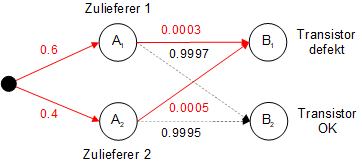
\includegraphics[width=0.5\textwidth]{Kapitel2/Bilder/image12}}
  \caption{Ereignisbaum zur Liefersituation der Transistoren}
  \label{fig:LiefersituationTransistoren}
\end{figure}

\noindent Es soll die Wahrscheinlichkeit f\"{u}r den Einbau eines defekten Transistors berechnet werden, also die Wahrscheinlichkeit, mit der das Ereignis $B_{1}$ eintritt. In dem Ereignisbaum in Bild \ref{fig:LiefersituationTransistoren} ist zu erkennen, dass das Ereignis $B_{1}$ auf zwei Pfaden erreicht wird, die in rot eingezeichnet sind. Die Berechnung erfolgt mit dem Satz der totalen Wahrscheinlichkeit zu

\begin{equation}\label{eq:twoeighty}
P(B_{1})=P(B_{1} |A_{1})\cdot P(A_{1})+P(B_{1} |A_{2})\cdot P(A_{2})=0.0003\cdot 0.6+0.0005\cdot 0.4=0.00038
\end{equation}

\noindent Die Wahrscheinlichkeit, dass ein defekter Transistor eingebaut wird, betr\"{a}gt somit 380 ppm.\bigskip

{\fontfamily{phv}\selectfont
\noindent\textbf{Satz von Bayes}} \smallskip

\noindent Die Berechnung der Wahrscheinlichkeit $P(B|A)$ f\"{u}r ein Ereignis B unter der Bedingung, dass ein Ereignis A eingetroffen ist, ist teilweise einfacher zu berechnen als die Wahrscheinlichkeit $P(B|A)$. Durch Anwendung der Regeln f\"{u}r die bedingte Wahrscheinlichkeit aus Gleichung \eqref{eq:twosixty}

\begin{equation}\label{eq:twoeightyone}
P(B|A)\cdot P(A)=P(A|B)\cdot P(B)
\end{equation}

\noindent ergibt sich die Wahrscheinlichkeit $P(B|A)$ aus der Wahrscheinlichkeit $P(B|A)$ zu

\begin{equation}\label{eq:twoeightytwo}
P(A|B)=\dfrac{P(B|A)\cdot P(A)}{P(B)}
\end{equation}

\noindent Wird die Wahrscheinlichkeit P(B) ausgedr\"{u}ckt \"{u}ber die totale Wahrscheinlichkeit, ergibt sich der Satz von Bayes. 

\begin{equation}\label{eq:twoeightythree}
P(A|B)=\dfrac{P(B|A)\cdot P(A)}{P(B)} =\dfrac{P(B|A)\cdot P(A)}{\sum _{n=1}^{N}P(B|A_{n}) \cdot P(A_{n})}
\end{equation}

\noindent
\colorbox{lightgray}{%
\arrayrulecolor{white}%
\renewcommand\arraystretch{0.6}%
\begin{tabular}{ wl{16.5cm} }
{\fontfamily{phv}\selectfont
\noindent{Beispiel: Zulieferer und Defekte von Transistoren}}
\end{tabular}%
}\bigskip

\noindent Als Anwendung des Satzes von Bayes wird die Frage diskutiert, mit welcher Wahrscheinlichkeit ein eingebauter defekter Transistor von Zulieferer 2 stammt, wenn die im vorigen Beispiel beschriebene Situation vorliegt. Die Berechnung der gesuchten Wahrscheinlichkeit $P(A{}_{2}|B{}_{1})$ erfolgt \"{u}ber den Satz von Bayes zu

\begin{equation}\label{eq:twoeightyfour}
\begin{split}
P(A_{2} |B_{1} ) & =\dfrac{P(B_{1} |A_{2} )\cdot P(A_{2} )}{P(B_{1} )} \\ 
& =\dfrac{P(B_{1} |A_{2})\cdot P(A_{2})}{\sum _{n=1}^{2}P(B_{1} |A_{n} ) \cdot P(A_{n})} =\dfrac{0.0005\cdot 0.4}{0.0003\cdot 0.6+0.0005\cdot 0.4}=52.63 \%
\end{split}
\end{equation}

\noindent Unter der Bedingung, dass ein defekter Transistor vorliegt, stammt er mit einer Wahrscheinlichkeit von 52.63 \% von Zulieferer 2, obwohl dieser weniger Transistoren liefert als Zulieferer 1.\bigskip

{\fontfamily{phv}\selectfont
\noindent\textbf{Zusammenfassung der S\"{a}tze zur Wahrscheinlichkeit nach Kolmogoroff}} \smallskip

\noindent Tabelle \ref{tab:twosix} fasst die S\"{a}tze zur Wahrscheinlichkeit nach Kolmogoroff zusammen.

\begin{table}[H]
\setlength{\arrayrulewidth}{.1em}
\caption{Tabellarische \"{U}bersicht der an der \"{U}bertragungsfunktion ablesbaren Systemeigenschaften}
\setlength{\fboxsep}{0pt}%
\colorbox{lightgray}{%
\arrayrulecolor{white}%
\begin{tabular}{| c | c |}
\hline
\parbox[c][0.35in][c]{3.3in}{\smallskip\centering\textbf{\fontfamily{phv}\selectfont{Regel}}} & 
\parbox[c][0.35in][c]{3.3in}{\smallskip\centering\textbf{\fontfamily{phv}\selectfont{Rechenvorschrift}}}\\ \hline

\parbox[c][0.4in][c]{3.3in}{\centering\fontfamily{phv}\selectfont{Additionssatz}} & 
\parbox[c][0.4in][c]{3.3in}{\centering\fontfamily{phv}\selectfont{$P(A\cup B)=P(A)+P(B)-P(A\cap B)$}}\\ \hline

\parbox[c][0.4in][c]{3.3in}{\centering\fontfamily{phv}\selectfont{Additionssatz komplementärer Ereignisse}} & 
\parbox[c][0.4in][c]{3.3in}{\centering\fontfamily{phv}\selectfont{$P(A)+P(A)=1$}}\\ \hline

\parbox[c][0.4in][c]{3.3in}{\centering\fontfamily{phv}\selectfont{Additionssatz unabh\"{a}ngiger Ereignisse}} & 
\parbox[c][0.4in][c]{3.3in}{\centering{\fontfamily{phv}\selectfont{$P\left(A_{1} \cup ...\cup A_{N} \right)=P(A_{1} )+...+P(A_{N})$}}}\\ \hline

\parbox[c][0.5in][c]{3.3in}{\centering\fontfamily{phv}\selectfont{Bedingte Wahrscheinlichkeit}} & 
\parbox[c][0.5in][c]{3.3in}{\centering{\fontfamily{phv}\selectfont{$P(A|B)=\dfrac{P(A\cap B)}{P(B)}$}}}\\ \hline

\parbox[c][0.5in][c]{3.3in}{\centering\fontfamily{phv}\selectfont{Multiplikationssatz}} & 
\parbox[c][0.5in][c]{3.3in}{\centering\fontfamily{phv}\selectfont{$P(A\cap B)=P(A|B)\cdot P(B)=P(B|A)\cdot P(A)$}}\\ \hline

\parbox[c][0.7in][c]{3.3in}{\centering\fontfamily{phv}\selectfont{Statistische Unabh\"{a}ngigkeit}} & 
\parbox[c][0.7in][c]{3.3in}{\centering\fontfamily{phv}\selectfont{$P(A|B)=P(A)$ \\ $P(B|A)=P(B)$ \\ $P(A\cap B)=P(A)\cdot P(B)$}}\\ \hline

\parbox[c][0.55in][c]{3.3in}{\centering\fontfamily{phv}\selectfont{Totale Wahrscheinlichkeit}} & 
\parbox[c][0.55in][c]{3.3in}{\centering\fontfamily{phv}\selectfont{$P(B)=\sum _{n=1}^{N}P(B|A_{n}) \cdot P(A_{n})$}}\\ \hline

\parbox[c][0.55in][c]{3.3in}{\centering\fontfamily{phv}\selectfont{Satz von Bayes}} & 
\parbox[c][0.55in][c]{3.3in}{\centering\fontfamily{phv}\selectfont{$P(A|B)=\dfrac{P(B|A)\cdot P(A)}{\sum _{n=1}^{N}P(B|A_{n} ) \cdot P(A_{n})}$}}\\ \hline

\end{tabular}%
}
\label{tab:twosix}
\end{table}
 
\noindent Mit den Regeln und Beispielen aus diesem Kapitel ist der Begriff der Wahrscheinlichkeit eingef\"{u}hrt. Au{\ss}erdem sind grundlegende Rechenregeln zur Berechnung der Wahrscheinlichkeit bekannt, sie werden im Folgenden in einem Projekt angewandt.

\clearpage

\subsection{Anwendungsbeispiel: Sensordiagnose im Steuerger\"{a}t}

\noindent Zur Erkennung von Sensorfehlern werden in Steuerger\"{a}ten Diagnoseverfahren eingesetzt. Sie \"{u}berwachen Ausgangsspannungen von Sensoren und plausibilisieren unterschiedliche Sensorsignale miteinander.

\noindent 
\begin{figure}[H]
  \centerline{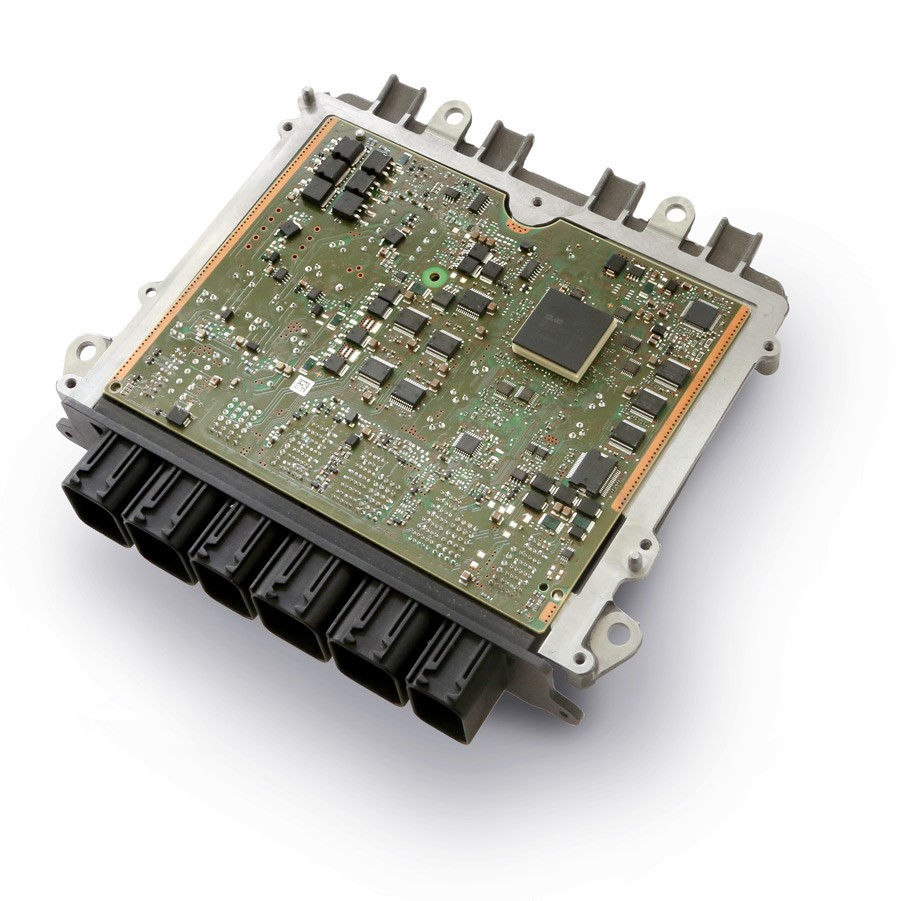
\includegraphics[width=0.5\textwidth]{Kapitel2/Bilder/image13}}
  \caption{Motorsteuerger\"{a}t}
  \label{fig:Motorsteuergeraet}
\end{figure}

\noindent Diagnosefunktionen sollten idealerweise so arbeiten, dass sie eine Fehlfunktion erkennen, wenn sie tats\"{a}chlich vorliegt und nicht reagieren, wenn der entsprechende Sensor nicht fehlerhaft ist. Die Diagnose von Fehlern ist jedoch nicht ideal. Reale Diagnosekonzepte haben eine endliche Aussagesicherheit. Die Auswirkungen werden im Folgenden mithilfe der Wahrscheinlichkeitsrechnung analysiert.\newline

\noindent Von einer Diagnosefunktion ist bekannt, dass sie mit einer Wahrscheinlichkeit von 99.99 \% einen defekten Sensor als defekt erkennt. Au{\ss}erdem ist bekannt, dass mit einer Wahrscheinlichkeit von 0.02~\% funktionsf\"{a}hige Sensoren als defekt eingestuft werden. Au{\ss}erdem ist aus einer Ausfallstatistik bekannt, dass die Wahrscheinlichkeit f\"{u}r einen Sensordefekt bei 100 ppm liegt. \newline

\noindent Es wird die Frage diskutiert, mit welcher Wahrscheinlichkeit ein Sensor wirklich defekt ist, wenn er mit der oben diskutierten Diagnosefunktion als defekt erkannt wurde. Um die Aufgabe zu l\"{o}sen, werden zu Beginn zwei Ereignisse definiert:

\begin{itemize}
    \item Ereignis A: Sensor ist defekt
    \item Ereignis B: Diagnoseergebnis ist positiv, Sensor wird als defekt eingestuft
\end{itemize}

\noindent Die Aufgabenstellung kann auch mithilfe eines Ereignisbaumes wie in Bild \ref{fig:Sensordiagnose} beschrieben werden. An die entsprechenden Zweige werden die bekannten Wahrscheinlichkeiten gekennzeichnet. Da ein sicheres Ereignis S bei einem Experiment die Wahrscheinlichkeit 1 besitzt, sind auch die Wahrscheinlichkeiten der \"{u}brigen Zweige bekannt. 

\noindent 
\begin{figure}[H]
  \centerline{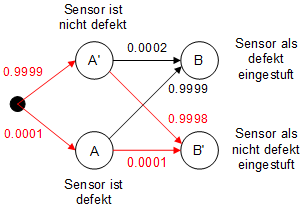
\includegraphics[width=0.4\textwidth]{Kapitel2/Bilder/image14}}
  \caption{Ereignisbaum zum Beispiel der Sensordiagnose}
  \label{fig:Sensordiagnose}
\end{figure}

\noindent In der Fragestellung ist die Wahrscheinlichkeit gesucht, mit der unter der Voraussetzung eines positiven Diagnoseergebnisses der Sensor tats\"{a}chlich defekt ist. Dies entspricht der bedingten Wahrscheinlichkeit $P(A|B)$. \newline

\noindent Bekannt ist die Wahrscheinlichkeit $P(B|A) = 99.99\%$, mit der ein defekter Sensor als defekt erkannt wird, und die Wahrscheinlichkeit $P(B|A') = 0.02\%$, mit der ein funktionst\"{u}chtiger Sensor als defekt eingestuft wird. Au{\ss}erdem betr\"{a}gt die Wahrscheinlichkeit f\"{u}r einen Sensordefekt $P(A) = 100ppm = 10^{-4}$.\newline

\noindent Da es sich um eine bedingte Wahrscheinlichkeit handelt, kann mit dem Satz von Bayes gearbeitet werden.

\begin{equation}\label{eq:twoeightyfive}
\begin{split}
P(A|B) & = \dfrac{P(B|A)\cdot P(A)}{P(B|A)\cdot P(A)+P(B|A')\cdot P(A')} \\ 
& = \dfrac{0.9999\cdot 10^{-4} }{0.9999\cdot 10^{-4} +0.0002\cdot \left(1-10^{-4} \right)}  = 33.33 \% 
\end{split}
\end{equation}

\noindent Im Folgenden soll die Vorgehensweise bei der Berechnung mit dem Ereignisbaum aus Bild \ref{fig:Sensordiagnose} gezeigt werden. Um die Wahrscheinlichkeit zu berechnen, mit der unter der Voraussetzung eines positiven Diagnoseergebnisses der Sensor tats\"{a}chlich defekt ist, muss der Ereignisbaum umgestellt werden.

\noindent 
\begin{figure}[H]
  \centerline{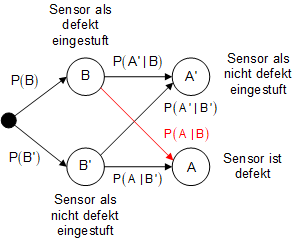
\includegraphics[width=0.4\textwidth]{Kapitel2/Bilder/image15}}
  \caption{Umgestellter Ereignisbaum zum Beispiel der Sensordiagnose}
  \label{fig:UmgestellterEreignisbaumSensordiagnose}
\end{figure}

\noindent Zur Berechnung der gesuchten Wahrscheinlichkeit muss zun\"{a}chst die Wahrscheinlichkeit f\"{u}r ein positives Testergebnis P(B) bestimmt werden. Mit dem Ereignisbaum aus Bild \ref{fig:Sensordiagnose} oder dem Satz der totalen Wahrscheinlichkeit folgt diese zu

\begin{equation}\label{eq:twoeightysix}
P(B)=P(B|A')\cdot P(A')+P(B|A)\cdot P(A)=0.0002\cdot 0.9999+0.9999\cdot 10^{-4} =3\cdot 10^{-4}
\end{equation}

\noindent Da die Wahrscheinlichkeit des Pfades 0-A-B im Ereignisbaum in Bild \ref{fig:Sensordiagnose} gleich der Wahrscheinlichkeit 0-B-A in Bild \ref{fig:UmgestellterEreignisbaumSensordiagnose} sein muss, kann die Wahrscheinlichkeit f\"{u}r einen defekten Sensor bei einem positiven Diagnoseergebnis berechnet werden. 

\begin{equation}\label{eq:twoeightyseven}
P(A|B)=\dfrac{P(B|A)\cdot P(A)}{P(B)} =\dfrac{0.9999\cdot 10^{-4} }{3\cdot 10^{-4} } = 33.33 \% 
\end{equation}

\noindent Bei n\"{a}herer Betrachtung entspricht diese Rechnung dem Satz von Bayes.\newline

\noindent Das Ergebnis der Berechnung besagt, dass trotz des positiven Diagnoseergebnisses die Wahrscheinlichkeit f\"{u}r einen Sensordefekt lediglich bei 33.33 \% liegt. Ursache daf\"{u}r ist, dass der Anteil funktionsf\"{a}higer Sensoren sehr gro{\ss} ist. In Bild \ref{fig:SensorDiagnose} ist diese Aussagesicherheit als Funktion der Wahrscheinlichkeit $P(B|A')$ dargestellt, mit der ein funktionst\"{u}chtiger Sensor als defekt eingestuft wird. Der in die Grafik eingezeichnete Punkt gibt das Ergebnis f\"{u}r $P(B|A') = 0.02 \%$ an.

\noindent 
\begin{figure}[H]
  \centerline{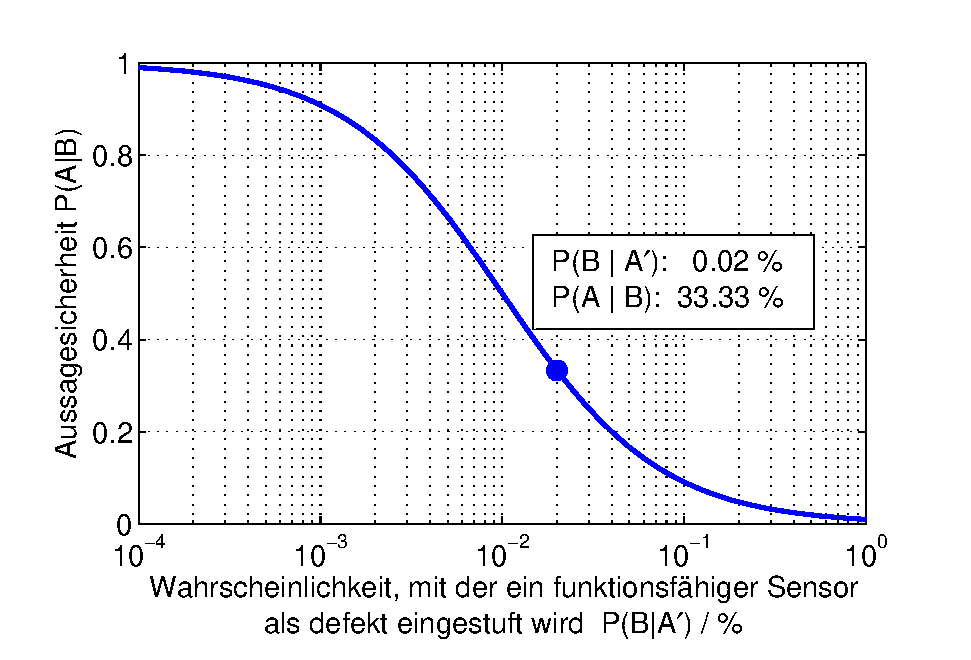
\includegraphics[width=0.5\textwidth]{Kapitel2/Bilder/image16}}
  \caption{Wahrscheinlichkeit mit der ein Sensor wirklich defekt ist, wenn er mit einer Diagnosefunktion als defekt eingestuft wurde}
  \label{fig:SensorDiagnose}
\end{figure}

\noindent Die Rechnung zeigt, dass sich die Wahrscheinlichkeit P(B{\textbar}A'), mit der ein funktionst\"{u}chtiger Sensor als defekt eingestuft wird, stark in das Ergebnis eingeht. Entwickler von Diagnosefunktionen sind deshalb bestrebt, gerade diesen Fehler zu minimieren.

\clearpage

\subsection{Literatur}


\begin{tabular}{|p{0.6in}|p{5.7in}|} \hline 
[Krey91] & Kreyszig, Erwin: Statistische Methoden und ihre Anwendungen\newline 4., unver\"{a}nderter Nachdruck der 7. Auflage\newline Vandenhoeck \& Ruprecht, G\"{o}ttingen, 1991 \\ \hline 
[Papu01] & Papula, Lothar: Mathematik f\"{u}r Ingenieure und Naturwissenschaftler Band 3\newline 4., verbesserte Auflage\newline Vieweg Teubner, Braunschweig / Wiesbaden, 2008 \\ \hline 
[Fahr06] & Fahrmeir, Ludwig; K\"{u}nstler, Rita; Pigeot, Iris; Tutz, Gerhard: Der Weg zur Datenanalyse\newline 6. Auflage\newline Springer Berlin Heidelberg New York, 2006 \\ \hline 
\end{tabular}
